\chapter{Experimentación}

% ------------------------------------------------------------------------------------------------------------
% ------------------------------------------------------------------------------------------------------------


\section{Problemas propuestos}

Como se ha mecionado anteriormente, y con el objetivo de validar los métodos de predicción conformal en diferentes tipos de problemas, este trabajo se centra en tres casuísticas que, si bien están relacionadas en el ámbito de la \acrshort{AF}, se tratan de diferente forma en el campo del \acrshort{ML}: 

\begin{enumerate}

    \item Estimación de la edad legal resuelta como un problema de regresión: El problema de \textbf{estimación de edad (\textit{age estimation})} consiste en predecir la edad cronológica de un individuo en una escala continua, lo que lo define como un problema de regresión.

    Para ello, se ha escogido usar las imágenes de radiografías maxilofaciales como entrada del algoritmo (véase la Figura \ref{fig:regression_problems}). Inicialmente se consideró incluir el sexo como metadato adicional en el modelo; sin embargo, se descartó tras observar de manera preliminar que no tenía un impacto significativo en el rendimiento del modelo, además de que su exclusión simplifica la arquitectura. 

    \todo{Para agosto: Un anexo que demuestre esto, yo ya lo he comprobado empíricamente}

    \begin{figure}[htbp]
        \centering
        \includegraphics[width=\textwidth]{capitulos/cap_04/imagenes/regression_problem.png}
        \caption[
            Esquema visual del modelos de regresión propuesto. 
        ]{
            Esquema visual del modelos de regresión propuesto. 
            El modelo solo tiene radiografías maxilofaciales como entrada. 
        } 
        \label{fig:regression_problems}
    \end{figure}
    
    \item Estimación de la mayoría de edad: Un problema inmediatamente derivado del anterior es la \textbf{estimación de mayoría de edad (\textit{age majority esimation})}, útil en contextos legales donde es necesario determinar si una persona ha alcanzado la mayoría de edad. Este se trata de un problema de clasificación binaria, en el que el objetivo es asignar a cada individuo una de dos clases: ``menor de edad'' o ``mayor de edad''.
    
    \item Estimación de la edad legal resuelta como un problema de clasificación multiclase: Se propone un problema de estimación de edad, pero planteado como problema de clasificación multiclase, donde cada edad ---como valor entero--- es una clase independiente. El potencial para aunar el planteamiento de un problema de regresión con uno de clasificación viene de la mano de la \acrshort{CP}, que, aplicada al problema de clasificación, permite generar conjuntos de etiquetas que toleran la cercanía entre clases, de forma que errores pequeños en el valor predicho (por ejemplo, predecir 19 en lugar de 20) no se consideren fallos completos.

\end{enumerate}

% ------------------------------------------------------------------------------------------------------------
% ------------------------------------------------------------------------------------------------------------

\section{Protocolo de validación experimental}

Como se ha descrito en el capítulo previo, se han proporcionado los datos ya dividos en conjunto de entrenamiento (\textit{train}) y de test, para evitar problemas asociados al \textit{data snooping}%
\footnote{
    El \textbf{\textit{data snooping}} ocurre cuando información del conjunto de test se filtra, directa o indirectamente, en el proceso de entrenamiento del modelo, lo que puede llevar a una sobreestimación del rendimiento y a modelos que no generalizan adecuadamente ante datos nuevos.
}.
Al proporcionar las particiones predefinidas, se garantiza que no haya contaminación entre los datos de entrenamiento y test, manteniendo así la validez de las métricas obtenidas en el test. 

Sin embargo, si se optimizan los parámetros del modelo durante el entrenamiento sin disponer de un conjunto independiente para evaluar su rendimiento, se corre el riesgo de sobreajustarse a los datos de entrenamiento. Es por ello que, además del conjunto de entrenamiento y test, es esencial tener un \textbf{conjunto de validación} independiente que permita evaluar el modelo durante su desarrollo, ajustar hiperparámetros y comparar diferentes configuraciones sin contaminar la evaluación final en el conjunto de test. Se consideró realizar validación cruzada (\textit{cross-validation}), pero debido al elevado coste computacional que implica, los resultados satisfactorios obtenidos mediante una simple partición de los datos (\textit{train/validation split}), se decidió prescindir de su aplicación.

En la Figura \ref{fig:data_split_base} podemos ver la división del \textit{dataset} planteada. Cabe comentar que la división se ha realizado de forma estratificada en base a la edad y el sexo%
\footnote{
    La estratificación se realizó en intervalos de medio año de edad y por sexo; por ejemplo, una instancia con edad 17.7 y sexo masculino se etiquetó como ``17.5\_M'', o una de edad 18.2 y sexo femenino como ``18.0\_F'.
}.

\begin{figure}[htbp]
    \centering
    \includegraphics[width=0.8\textwidth]{capitulos/cap_04/imagenes/data_split_base.png}
    \caption[
        Diagrama de división del \textit{dataset} en \textit{train}, \textit{validation} y \textit{test}.
    ]{
        Diagrama de división del \textit{dataset} en \textit{train}, \textit{validation} y \textit{test}. 
    } 
    \label{fig:data_split_base}
\end{figure}

Es importante destacar que esta división se mantiene constante en todos los experimentos y para todos los problemas planteados, asegurando que las mismas instancias permanezcan en los mismos subconjuntos. Esto permite garantizar que ningún modelo preentrenado reutilice datos previamente utilizados en etapas de validación o calibración, algo especialmente relevante dado que los problemas abordados están jerárquicamente relacionados (la clasificación de sexo y mayoría de edad se deriva directamente de la clasificación de mayoría de edad, que a su vez se deriva de la estimación de edad).

Sin embargo, al emplear métodos de calibración o predicción conformal, si usamos los mismos datos de entrenamiento para la calibración, las probabilidades o intervalos de predicción tenderán a ser optimistas, pues el modelo ha sido entrenado con esos datos \cite{niculescu2005}. Por tanto, para evitar el sobreajuste y garantizar validez estadística se requiere de un subconjunto de datos adicional: el \textbf{conjunto de calibración}. Se ha escogido destinar el  20\% de los ejemplos de entrenamiento para calibración, basándose en los resultados empíricos de \cite{sesia2020} (que recomienda dedicar entre un 10\% y 30\% de datos de entrenamiento a calibración), tal y como se muestra en la Figura \ref{fig:data_split_conformal}.

\begin{figure}[htbp]
    \centering
    \includegraphics[width=0.8\textwidth]{capitulos/cap_04/imagenes/data_split_conformal.png}
    \caption[
        Diagrama de división del \textit{dataset} en \textit{train}, \textit{validation}, \textit{calibration} y \textit{test}.
    ]{
        Diagrama de división del \textit{dataset} en \textit{train}, \textit{validation}, \textit{calibration} y \textit{test}. 
    } 
    \label{fig:data_split_conformal}
\end{figure}

Para una comparativa más justa entre los métodos que usan \acrshort{CP} y los que no, se utilizará la siguiente estrategia: los métodos que no emplean \acrshort{CP} seguirán el esquema tradicional de división de datos (en entrenamiento, validación y test), mientras que los métodos basados en \acrshort{CP} incorporarán además un conjunto de calibración independiente. Esta diferencia en el diseño experimental nos permitirá cuantificar cómo afecta a la capacidad predictiva de los modelos el hecho de reservar parte de los datos para el proceso de calibración.

% ------------------------------------------------------------------------------------------------------------
% ------------------------------------------------------------------------------------------------------------

\section{Preprocesado de los datos}

Dado que las imágenes del conjunto de datos disponible son significativamente más anchas que altas, se han normalizado todas las dimensiones a 448×224 píxeles para homogenizar las entradas del modelo%
\footnote{
    El redimensionado se aplicó de forma consistente a todo el conjunto (entrenamiento, validación, calibración y test), utilizando interpolación bilineal.
}.
También se ha realizado \textit{data augmentation} en el conjunto de entrenamiento, introduciendo
transformaciones aleatorias en cada época para simular condiciones de posicionamiento del paciente y de la 
máquina o iluminación ligeramente variable:
\begin{itemize}
    \item volteo horizontal en la mitad de las imágenes,
    \item rotación entre -3 y 3 grados,
    \item traslaciones de hasta el 2\%,
    \item escalado entre el 95 y 105\%, y
    \item cambios de brillo y contraste entre 80 y 120\%. 
\end{itemize}

Se ha establecido un tamaño de \textit{batch} de 32, tras encontrar preeliminarmente un equilibrio entre 
regularización y buen ritmo de aprendizaje.

% ------------------------------------------------------------------------------------------------------------
% ------------------------------------------------------------------------------------------------------------

\section{Esquema general de los experimentos realizados}

Para cada problema planteado, se propone realizar una comparativa entre distintos métodos, incluyendo tanto predicciones puntuales como interválicas en los casos de regresión, y predicciones de una sola etiqueta o de un conjunto de etiquetas en los casos de clasificación, utilizando tanto heurísticas como métodos de \acrshort{CP}. De esta forma queremos evaluar tanto la utilidad tradicional para estimar el valor esperado como la capacidad para proporcionar intervalos de confianza fiables que capturen la incertidumbre predictiva. Todas las métricas se calculan sobre el conjunto de test. 

Se requerirá el 95\% de confianza en las predicciones interválicas o de conjunto de etiquetas, que es la cifra de confianza generalmente empleada en \acrshort{AF}. 

\subsection{Problema de estimación de edad}

Para el problema de estimación de edad se han propuesto los siguientes cuatro métodos (véase la Figura \ref{fig:AE_experimental_pipeline}):

\begin{itemize}

    \item \textbf{Método `base'}: Se trata de un modelo de regresión puntual sin técnicas de \acrshort{CP}. La predicción interválica se construirá con la predicción puntual $\pm$ 2 veces el error absoluto medio obtenido en el conjunto de validación, que es una aproximación heurística común para construir intervalos de predicción que no asumen una distribución de errores específica. Este método sirve como \textit{baseline} para comparar la mejora que aportan técnicas más sofisticadas.

    \item \textbf{Método `ICP'}: Implementa el método \textit{Inductive Conformal Prdiction} para la \acrshort{CP}. 
    
    \item \textbf{Método `QR'}: Este método implementa \textit{Quantile Regression}. Utiliza tres cuantiles 
    $$
    [0.5, \alpha/2, 1-\alpha/2]
    $$ 
    para predecir la predicción puntual, límite inferior y límite superior, respectivamente.

    \item \textbf{Método `CQR'}: Este método implementa \textit{Conformalized Quantile Regression}, con los mismos cuantiles que \acrshort{QR}. 

\end{itemize} 

Para cada método se han entrenado 10 modelos independientes desde cero, con el objetivo de capturar la variabilidad inherente al proceso de entrenamiento.


% ------------------------------------------------------------------------------------------------------------

\subsection{Problema de clasificación de mayoría de edad}

Respecto al problema de clasificación de mayoría de edad, se han propuesto los siguientes tres métodos (veáse la Figura \ref{fig:AMM_experimental_pipeline}): 

\begin{itemize}

    \item \textbf{Método `base'}: Se trata del modelo de clasificación de una sola etiqueta sin uso de técnicas de \acrshort{CP}. El conjunto de predicción se considerará aquel formado exclusivamente por la clase más probable. El entrenamiento de este modelo partirá de un modelo `base' ya entrenado para el problema de estimación de edad, al cual se realizará un \textit{fine-tuning} de la cabecera. Este método sirve de \textit{baseline} para comparar con el resto. 

    \item \textbf{Método `LAC'}: Este método implementa la técnica \acrshort{LAC} para \acrshort{CP}. El entrenamiento del modelo partirá de un modelo \acrshort{ICP} ya entrenado para regresión.

    \item \textbf{Método `MCM'}: Este método implementa la técnica MCM para CP. El modelo será exactamente el mismo que el de \acrshort{LAC}. Solo cambiará la calibración e inferencia conformal. 

\end{itemize} 

No se han implementado las técnicas \acrshort{APS} y \acrshort{RAPS} de \acrshort{CP} para clasificación, ya que \acrshort{APS} es teóricamente equivalente a \acrshort{LAC} en problemas de clasificación binaria, y \acrshort{RAPS} no resulta aplicable en dicho contexto.

En este caso, también se han obtenido 10 modelos independientes para cada método. 

% ------------------------------------------------------------------------------------------------------------

\subsection{Problema de clasificación de edad}

% Al igual que en el problema de AAM, para el problema de AMSC se ha seguido la misma lógica de evaluación, aplicando tanto predicción puntual como técnicas de CP para obtener conjuntos de predicción. 

% \todo{
%     No me gusta mucho usar estas siglas en el texto, no sé si debería directamente eliminarlas del trabajo o solo dejarlas para usar en los resultados (para tablas y gráficos, donde no cabe mucho texto)
% }


Para el problema de clasificación de edad, se ha empleado la técnica de calibración de probabilidades \textit{Temperature Scaling} para ajustar las salidas del modelo de clasificación multiclase, con el objetivo de mejorar la calidad de las probabilidades utilizadas durante la fase de inferencia conformal. Esta calibración probabilística se realiza antes del \textit{softmax}. Se ha optado por utilizar el conjunto de validación para llevar a cabo dicha calibración de probabilidades, dado que, aunque no es el enfoque más riguroso ---ya que lo ideal sería dividir el conjunto de calibración en dos subconjuntos independientes, uno para la calibración de probabilidades y otro para la calibración conformal--- esta estrategia mostró buenos resultados en la práctica. Esto se debe a que el conjunto de validación empleado era suficientemente representativo y permitió obtener probabilidades calibradas de manera adecuada. Esta calibración probabilística no afecta a la variabilidad entre modelos con los mismos parámetros, dado que el algoritmo es determinista y produce resultados consistentes para un mismo conjunto de datos y parámetros. 

Los métodos propuestos para este problema son (véase la Figura \ref{fig:AGC_experimental_pipeline}):

\begin{itemize}

    \item \textbf{Método `base'}: Al igual que para el problema de clasificación de mayoría de edad, funciona como un clasificador normal sin métodos de \acrshort{CP}, y se usa de \textit{baseline} para comparar con el resto. El entrenamiento de este modelo partirá de un modelo `base' ya entrenado para el problema de AMM.

    \item \textbf{Método `LAC'}: Este método implementa la técnica LAC para \acrshort{CP}. El entrenamiento de este modelo partirá del modelo \acrshort{LAC} ya entrenado para el problema de AMM.

    \item \textbf{Método `MCM'}: Implementa la técnica \acrshort{MCM} para \acrshort{CP}. El modelo será exactamente el mismo que el de LAC para este mismo problema. 

    \item \textbf{Método `APS'}: Implementa la técnica \acrshort{APS} para \acrshort{CP}, con componente aleatoria para tamaños de conjunto de predicción más ajustados. El modelo será exactamente el mismo que el de LAC para este mismo problema.

    \item \textbf{Método `RAPS'}: Implementa la técnica \acrshort{RAPS} para \acrshort{CP}, también con componente aleatoria. El modelo será exactamente el mismo que el de LAC para este mismo problema. 
    
    \item \textbf{Método `SAPS'}: Implementa la técnica \acrshort{SAPS} para \acrshort{CP}. Usará el mismo modelo que \acrshort{LAC}. 

\end{itemize} 


% \begin{landscape}
%     \thispagestyle{fancy}
%     \begin{figure}[htbp]
%         \centering
%         \includegraphics[width=0.75\linewidth]{capitulos/cap_05/imagenes/AE_experimental_pipeline.png}
%         \captionsetup{width=0.75\linewidth}
%         \caption[
%             Esquema de experimentación para la estimación de edad.
%         ]{
%             Esquema de experimentación para la estimación de edad. Cada modelo se entrena por separado. `R' se refiere a `Regresión puntual' (de una sola neurona de salida), `QR' a Quantile Regression , `ICP' a Inductive Conformal Prediction y `CQR' a Conformalized Quantile Regression.
%         } 
%         \label{fig:AE_experimental_pipeline}
%     \end{figure}
% \end{landscape}

% \thispagestyle{fancy}
\begin{landscape}
\thispagestyle{fancy}

\begin{figure}[H]
    \centering
    \begin{minipage}{0.53\linewidth}
        \includegraphics[width=1.3\textwidth]{capitulos/cap_05/imagenes/AE_experimental_pipeline.png}
    \end{minipage}%
    \hfill
    \begin{minipage}{0.3\linewidth}
        \caption[
            Esquema de experimentación para la estimación de edad.
        ]{
            Esquema de experimentación para la estimación de edad. 
            Cada modelo se entrena por separado. 
            
            R: Regresión puntual
            
            QR: Quantile Regression 
            
            ICP: Inductive Conformal Prediction 
            
            CQR: Conformalized Quantile Regression
        }
        \label{fig:AE_experimental_pipeline}
    \end{minipage}
\end{figure}


% \begin{figure}[H] 
%     \centering 
%     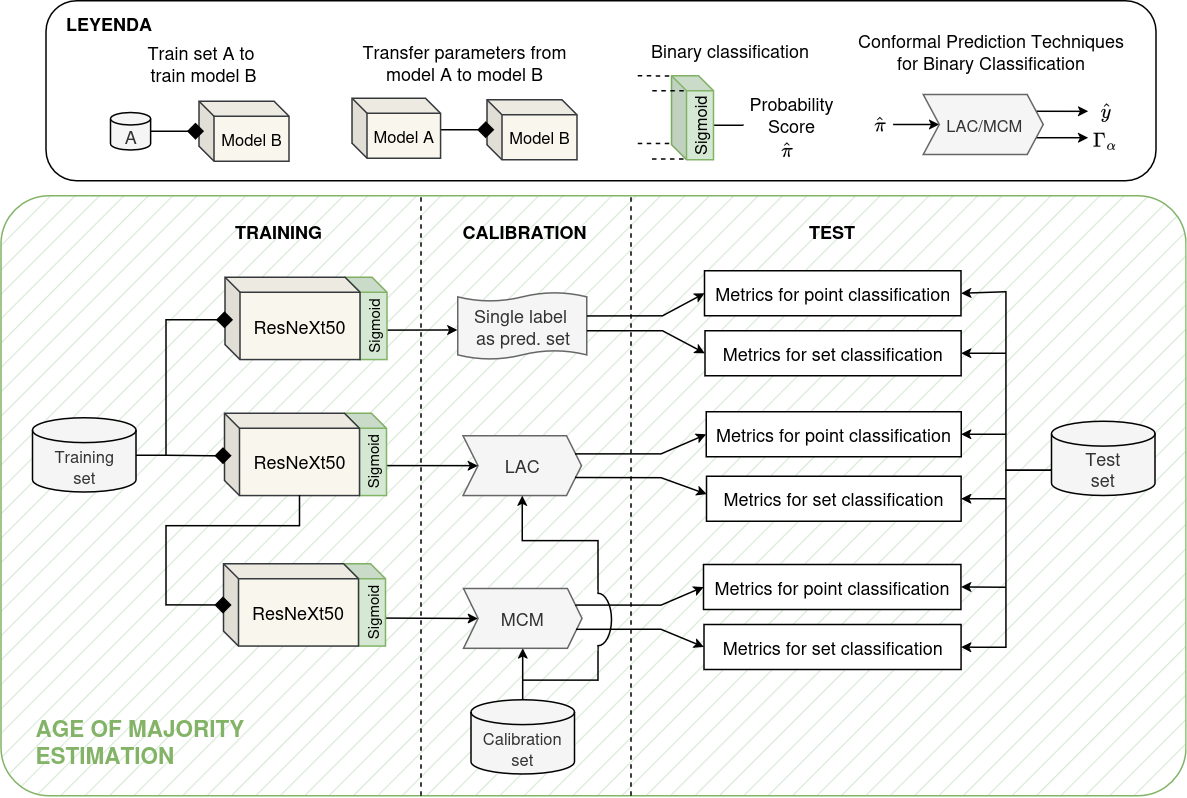
\includegraphics[width=1.3\textwidth]{capitulos/cap_05/imagenes/AMM_experimental_pipeline.png} 
%     \caption[ 
%         Esquema de experimentación para la clasificación de mayoría de edad. 
%     ]{ 
%         Esquema de experimentación para la clasificación de mayoría de edad. 

%         LAC: Least-Ambiguous set-valued Classifiers

%         MCM: Mondrian Confidence Machine
%     } 
%     \label{fig:AMM_experimental_pipeline} 
% \end{figure}





\begin{figure}[H]
    \raggedleft
    % --- Bloque con la imagen ---
    \begin{minipage}{0.51\linewidth}
        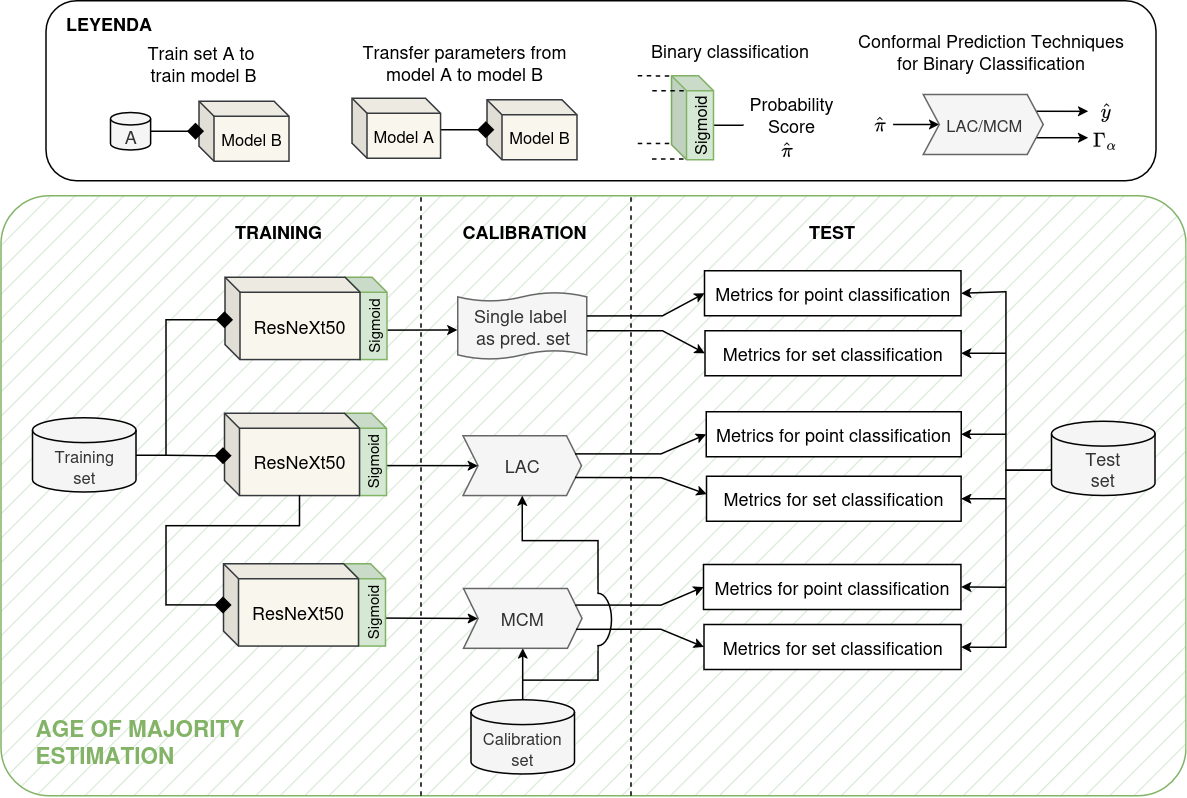
\includegraphics[width=1.3\linewidth]{capitulos/cap_05/imagenes/AMM_experimental_pipeline.png}
    \end{minipage}%
    \hfill
    % --- Bloque con el caption ---
    \begin{minipage}{0.33\linewidth}
        \caption[ 
            Esquema de experimentación para la clasificación de mayoría de edad. 
        ]{ 
            Esquema de experimentación para la clasificación de mayoría de edad. 

            LAC: Least-Ambiguous set-valued Classifiers

            MCM: Mondrian Confidence Machine
        } 
        \label{fig:AMM_experimental_pipeline}
    \end{minipage}
\end{figure}


\begin{figure}[H]
    \raggedleft
    % --- Bloque con la imagen ---
    \begin{minipage}{0.5\linewidth}
        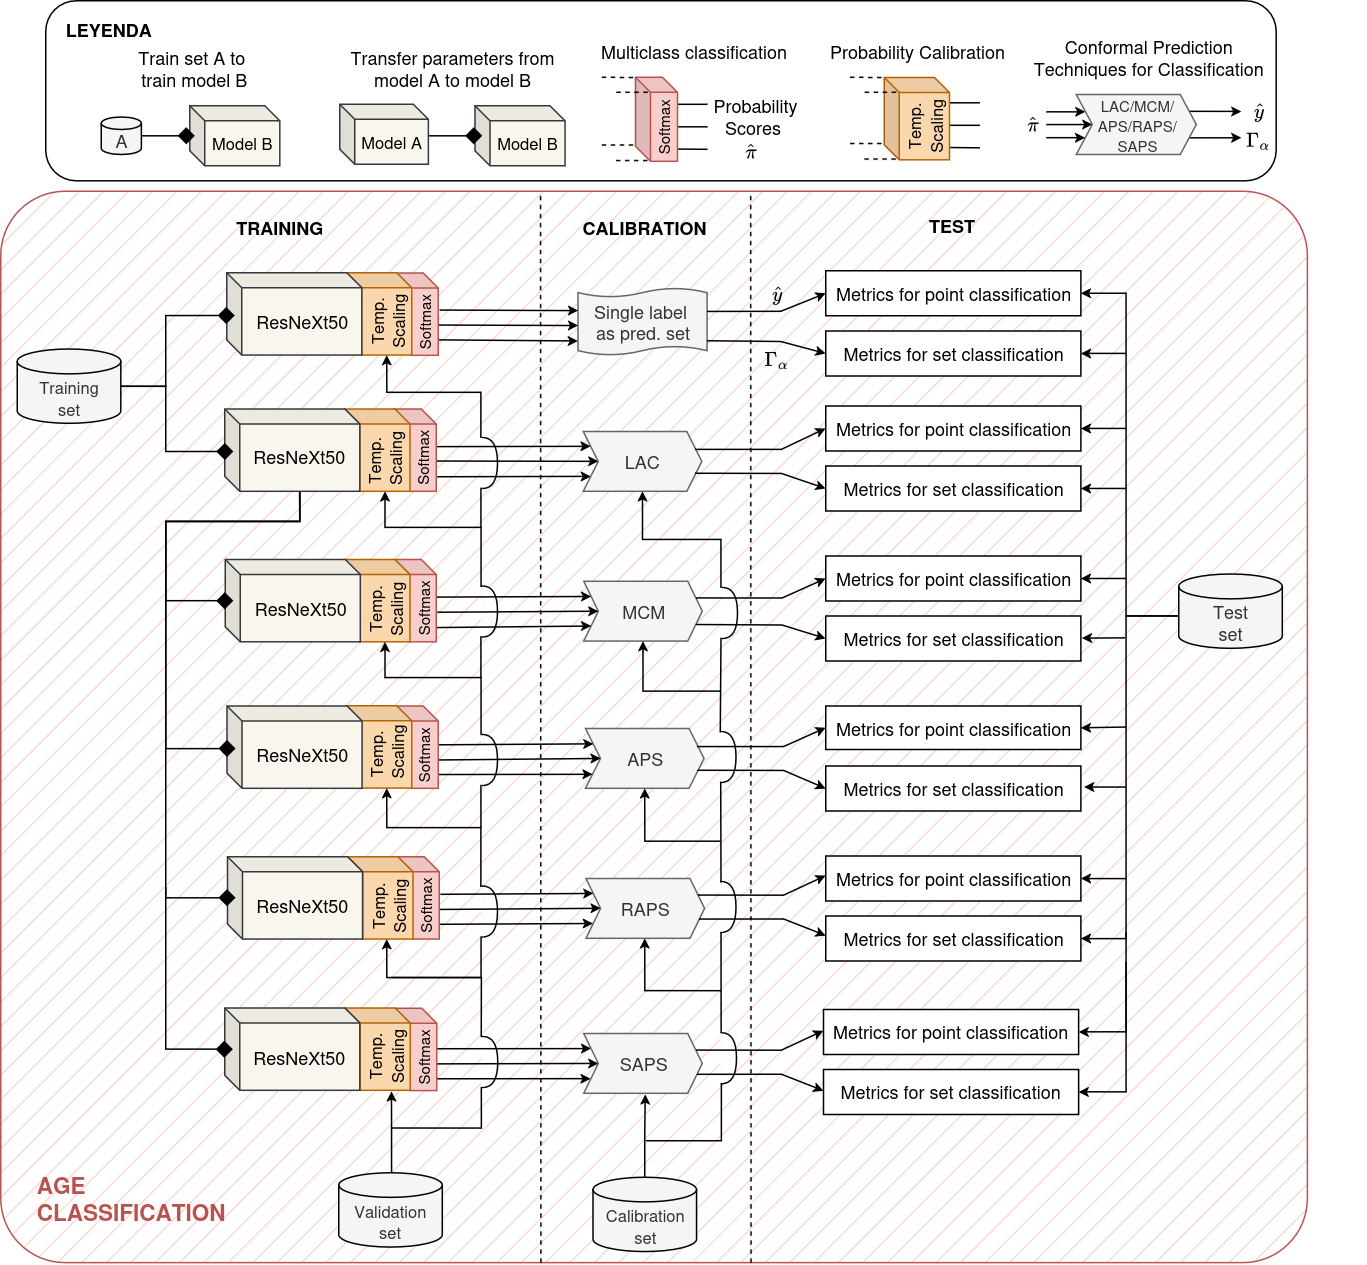
\includegraphics[width=1.3\linewidth]{capitulos/cap_05/imagenes/AGC_experimental_pipeline.png}
    \end{minipage}%
    \hfill
    % --- Bloque con el caption ---
    \begin{minipage}{0.36\linewidth}
        \caption[
            Esquema de experimentación para la clasificación de edad. 
        ]{
            Esquema de experimentación para la clasificación de edad. 

            LAC: Least-Ambiguous set-valued Classifiers

            MCM: Mondrian Confidence Machine

            APS: Adaptive Prediction Sets

            RAPS: Regularized Adaptive Prediction Sets

            SAPS: Sorted Adaptive Prediction Sets

            Temp. Scaling: Temperature Scaling
        }
        \label{fig:AGC_experimental_pipeline}
    \end{minipage}
\end{figure}

\end{landscape}

\FloatBarrier

\thispagestyle{fancy}


% ------------------------------------------------------------------------------------------------------------
% ------------------------------------------------------------------------------------------------------------

\section{Evaluación del rendimiento}


\subsection{Métricas para regresión}

En nuestro problema de regresión emplearemos dos tipos de métricas con el objetivo de evaluar aspectos distintos del desempeño del modelo.

Por una parte, las métricas destinadas a las predicciones puntuales se basan fundamentalmente en medir el error entre el valor real ($y_i$) y el valor esperado predicho ($\hat{y_i}$). Estas métricas nos permiten cuantificar directamente la discrepancia entre las estimaciones del modelo (estimación central en modelos de predicción interválica) y la \textit{ground truth}. Las métricas que empleamos para estas predicciones son:

\begin{itemize}
    \item El \textbf{error absoluto medio (\textit{mean absolute error}, MAE)} mide el promedio de las diferencias absolutas entre los valores reales ($Y_i$) y los valores predichos ($\hat{Y_i}$) por el modelo.

    $$
    MAE = \frac{1}{n} \sum_{i=1}^n{|y_i - \hat{y_i}|} \in [0, \infty)
    $$

    donde $n$ es el número de ejemplos/instancias con las que se cuenta en los datos a evaluar.

    La interpretación más inmediata de esta métrica es que representa cuánto se desvía en promedio la predicción del valor real sin considerar la dirección del error (positivo o negativo) y, por tanto, cuanto más se acerque a cero el valor, mejor es el ajuste del modelo.

    \item El \textbf{error cuadrático medio (\textit{mean squared error}, MSE)} mide el promedio de los errores al cuadrado entre valores reales ($Y_i$) y los valores predichos ($\hat{Y_i}$) por el modelo.
    
    $$
    MSE = \frac{1}{n} \sum_{i=1}^n{(y_i - \hat{y_i})^2} \in [0, \infty)
    $$

    Al igual que el MAE, cuantifica qué tan cerca están las predicciones de los valores reales, pero penaliza más los errores grandes, y es más sensible por tanto a valores atípicos.

\end{itemize}


Por otra parte, las métricas aplicadas a las predicciones interválicas examinan tanto la capacidad del modelo para abarcar el valor real dentro del intervalo predicho ---conocida como \textbf{cobertura (\textit{coverage})}--- como la \textbf{amplitud} del mismo, que es el ancho del rango de valores del intervalo de predicción. Generalmente, existe un compromiso entre ambos aspectos: al aumentar la amplitud, es más probable que el intervalo contenga el valor real, pero esto disminuye la precisión y utilidad práctica de la predicción. Veamos las métricas para este tipo de predicciones: 

\begin{itemize}
    \item La \textbf{cobertura empírica (\textit{empirical coverage})} cuantifica la proporción de valores reales dentro de los intervalos de predicción obtenidos. 
    
    $$
    EC = \frac{1}{n} 
        \sum_{i=1}^n{ \mathbb{I} \left[ l_i \le y_i \le u_i \right] } 
            \in \left[0, 1\right]
    $$

    donde $l_i$ y $u_i$ son los límites inferior y superior, respectivamente, de los intervalos de predicción obtenidos mediante inferencia conformal.

    Cuanto mayor sea el valor, mejor cobertura ofrece el modelo, si bien coberturas altas suelen conllevar intervalos excesivamente amplios, lo que reduce su utilidad práctica. Es por ello que, empleando métodos de \acrshort{CP}, tiene más sentido que el objetivo sea acercarse lo máximo posible a la cobertura marginal nominal ($1-\alpha$), garantizando así intervalos de predicción que equilibren precisión y fiabilidad sin ser inneceseriamente conservadores. 
    
    \item El \textbf{tamaño medio de intevalo de predicción (\textit{mean prediction inteval width})} mide qué tan amplios son en promedio los intervalos predichos.
    
    $$
    MPIW = \frac{1}{n} \sum_{i=1}^n{ \left( u_i - l_i \right) } \in (0, +\infty)
    $$
    
    Se desea matener este valor lo más pequeño posible, dado un nivel de cobertura adecuado. Valores altos indican intervalos anchos y, por tanto, poco útiles para la toma de decisiones. 

    \item La \textbf{\textit{mean interval score}} \cite{gneiting2007} trata de unificar en una sola métrica el \textit{trade-off} cobertura vs. amplitud del intervalo. Su expresión es la siguiente:

    \begin{align*} 
    MIS = \frac{1}{n} \sum_{i=1}^n
    \biggl( (u_i-l_i) \biggr.&+ \frac{2}{\alpha} \left( l_i-y_i \right) \mathbb{I}\left[ y_i<l_i \right] \\
    &+\left. \frac{2}{\alpha}  \left( y_i-u_i \right) \mathbb{I}\left[ y_i>u_i \right] \right)
    \in \left( 0, +\infty \right)
    \end{align*}

    Al igual que con el \textit{mean interval width}, una puntuación más baja en el \textit{mean interval score} indica un mejor rendimiento del modelo. El primer término ($u_i-l_i$) representa directamente la amplitud de cada intervalo, mientras que el segundo y tercer términos:

    \begin{itemize}
        \item $\frac{2}{\alpha} \left( l_i-y_i \right) \mathbb{I}\left[ y_i<l_i \right]$ penaliza los casos en que el valor verdadero $y_i$ está por debajo del límite inferior $l_i$, proporcionalmente a la distancia del límite inferior al valor real ($l_i-y_i$).
        \item $\frac{2}{\alpha}  \left( y_i-u_i \right) \mathbb{I}\left[ y_i>u_i \right]$ penaliza los casos en que el valor verdadero $y_i$ está por encima del límite superior $u_i$, proporcionalmente a la distancia del límite superior al valor real ($y_i-u_i$).
    \end{itemize}

    Estos dos últimos términos aplican una penalización crecientemente severa cuando las predicciones no cubren el valor verdadero ---y lo hacen multiplicando por $2/\alpha$, lo que enfatiza aún más los errores externos a medida que disminuye $\alpha$, es decir, cuando se busca mayor confianza.

\end{itemize}

Y, finalmente, también añadiremos elementos visuales para valorar el desempeño de las predicciones interválicas:

\begin{itemize}

    \item \textbf{Gráfica de dispersión de Cobertura Empírica - Amplitud Media del Intervalo de Predicción}: Este gráfico permite visualizar el compromiso entre cobertura lograda y tamaño del intervalo. Un buen modelo debería situarse cerca del nivel de confianza objetivo con intervalos lo más cortos posible. 

    \item \textbf{Histograma de tamaños de intervalos}: Esto nos permitirá analizar la distribución de las longitudes de los intervalos predichos. Una concentración alrededor de valores bajos indica intervalos más informativos, mientras que una distribución amplia o con colas largas puede revelar incertidumbre elevada en ciertos casos. Esta visualización nos será útil para aquellas técnicas que ofrecen intervalos predictivos adaptativos. 
    
    Solo tiene sentido analizar el histograma para aquellos métodos que dan intervalos de predicción de tamaño variable, como es en nuestro caso \acrshort{QR} y \acrshort{CQR}. 

\end{itemize}

% ------------------------------------------------------------------------------------------------------------

\subsection{Métricas para clasificación}

Como con la regresión, diferenciaremos entre las métricas de clasificación de etiqueta única y las de múltiples etiquetas para valorar los conjuntos de predicciones obtenidos con las técnicas de \acrshort{CP}.

Para la clasificación de etiqueta única usaremos: 

\begin{itemize}

    \item La \textbf{matriz de confusión} es una herramienta fundamental que permite visualizar el rendimiento de modelos de clasificación, tanto binarios como multiclase. Esta muestra una tabla con tantas columnas y filas como clases haya. En un eje, se representan las clases reales (etiquetas verdaderas), y en el otro eje, las clases predichas por el modelo. Cada celda de la matriz indica la cantidad de ejemplos que pertenecen a una clase real específica y que han sido clasificados como una clase predicha específica (véase la Figura \ref{fig:conf_matrix_binary}). Idealmente, los valores se concentrarían en la diagonal principal, lo que indicaría que las predicciones coinciden con los valores reales. Prácticamente todas las métricas y visualizaciones parten de la información ofrecida en esta matriz. 

    \begin{figure}[htbp]
        \centering
        \includegraphics[width=0.6\textwidth]{capitulos/cap_02/imagenes/confusion_matrix_binary.png}
        \caption{
            Matriz de confusión para la estimación de sexo según el modelo \textit{random forest} propuesto en \cite{bidmos2023}.
        } 
        \label{fig:conf_matrix_binary}
    \end{figure}

    \item La \textbf{exactitud (\textit{accuracy})} es la proporción de instancias totales bien clasificadas. 
    
    % \begin{figure}[htbp]
    %     \centering
    
    %     \begin{subfigure}[b]{0.3\textwidth}
    %         \centering
    %         \includegraphics[width=\textwidth]{capitulos/cap_02/imagenes/confusion_matrix_binary_1.png}
    %         \caption{Sin información de sexo}
    %         \label{fig:conf_matrix_general}
    %     \end{subfigure}
    %     \hfill
    %     \begin{subfigure}[b]{0.3\textwidth}
    %         \centering
    %         \includegraphics[width=\textwidth]{capitulos/cap_02/imagenes/confusion_matrix_binary_2.png}
    %         \caption{Sexo femenino}
    %         \label{fig:conf_matrix_female}
    %     \end{subfigure}
    %     \hfill
    %     \begin{subfigure}[b]{0.3\textwidth}
    %         \centering
    %         \includegraphics[width=\textwidth]{capitulos/cap_02/imagenes/confusion_matrix_binary_3.png}
    %         \caption{Sexo masculino}
    %         \label{fig:conf_matrix_male}
    %     \end{subfigure}
    
    %     \caption[
    %         Matrices de confusión para la estimación de mayoría/minoría de edad según el modelo de 
    %         \cite{porto2020}.
    %     ]{
    %         Matrices de confusión para la estimación de mayoría/minoría de edad según el modelo de 
    %         \cite{porto2020}.
    %         Se representan los valores de cada celda en términos porcentuales de los ejemplos reales que hay 
    %         de cada clase ($< 18$ y $\ge 18$), lo que permite comparar la matriz de confusión general de todos 
    %         los ejemplos (\ref{sub@fig:conf_matrix_general}) con la de ejemplos se sexo femenino 
    %         (\ref{sub@fig:conf_matrix_female}) y sexo masculino (\ref{sub@fig:conf_matrix_male}), permitiendo 
    %         identificar posibles sesgos en el modelo respecto al género, y así realizar una evaluación más 
    %         precisa del rendimiento del modelo en diferentes subgrupos de la población.
    %     }
    %     \label{fig:conf_matrix_binary_relative}

    % \end{figure}

\end{itemize}


Por otro lado, para la clasificación multietiqueta emplearemos:

\begin{itemize}

    \item La \textbf{cobertura empírica (\textit{empirical coverage})}, de forma análoga a la regresión, mide la proporción de veces que la etiqueta verdadera está contenida dentro del conjunto predicho.

    $$
    EC = \frac{1}{n} \sum_{i=1}^{n} \mathbb{I}(y_i \in \Gamma_\alpha(x_i))
    $$

    Esta variable se puede obtener o bien en todos los ejemplos del conjunto, o en subpoblaciones específicas de este.

    % \item Se denomina \textbf{violación de la cobertura empírica (\textit{empirical coverage violation})} a la magnitud en que la cobertura empírica no alcanza el nivel de cobertura teórico deseado $1 - \alpha$, definida como:

    % $$
    % ECV = max \left\{ 0,(1-\alpha)-EC \right\}
    % $$

    % Este valor cuantifica cuánto se desvía el método de la garantía nominal
    % \footnote{
    %     Se denomina garantía de cobertura nominal al nivel de cobertura garantizado estadísticamente.
    % } 
    % cuando no se alcanza la cobertura esperada. Una violación igual a cero indica que el método cumple o supera el nivel de cobertura deseado.

    % Esta métrica se suele calcular sobre subconjuntos específicos del conjunto de instancias para evaluar la cobertura condicional, es decir, la calidad de la cobertura dentro de subpoblaciones del dominio.

    \item El \textbf{tamaño medio de conjunto de predicción (\textit{mean prediction set size})} mide cuántas etiquetas, en promedio, incluyen los conjuntos de predicción conformales $\Gamma_\alpha(x)$.

    $$
    MPSS = \frac{1}{n} \sum_{i=1}^n | \Gamma_\alpha(x_i) |
    $$

    % \item Gráfico de barras de violación de cobertura en base al tamaño del conjunto (inspirada en la métrica \textit{Each-Size Coverage Violation} propuesta en \cite{huang2023conformal}): En esta gráfica, para cada tamaño posible del conjunto de predicción, se calcula la violación de cobertura empírica correspondiente, es decir, cuánto se desvía la cobertura observada respecto al nivel nominal $(1 - \alpha)$. Esto permite visualizar en qué tamaños de conjunto el modelo tiende a fallar más en cuanto a cobertura, proporcionando una forma más detallada de analizar el comportamiento del método conforme más allá de la cobertura global.

    
\end{itemize}


Y, finalmente, también usaremos elementos visuales para valorar el desempeño de las predicciones interválicas, como pueden ser:

\begin{itemize}

    \item \textbf{Gráfica de dispersión de Cobertura Empírica - Tamaño Medio del Conjunto de Predicción}: Este gráfico permite visualizar el compromiso entre cobertura lograda y tamaño del intervalo. Un buen modelo debería situarse cerca del nivel de confianza objetivo con intervalos lo más cortos posible. 

    \item \textbf{Histograma de tamaños de conjuntos de predicción}: De similar forma a como se plantean los histogramas de amplitudes de intervalos para regresión, se puede plantear histograma donde cada tamaño es el número de clases del conjunto predicho. Este nos permite ver la distribución de tamaños de conjuntos de predicción. Aquellos con pocas clases serán más informativos, mientras que tamaños más grnades pueden revelar una incertidumbre elevada.
    
\end{itemize}

% ------------------------------------------------------------------------------------------------------------

\subsection{Tests estadísticos}

En los casos en los que las diferencias en una métrica entre métodos presenten valores intercalados o solapamientos aparentes, se aplican tests estadísticos para determinar si las diferencias observadas son significativas, evitando basarnos únicamente de la comparación visual de medias o medianas.

En el análisis de comparación de métodos de predicción, se seleccionaron diferentes pruebas estadísticas según el cumplimiento de los supuestos de normalidad y homocedasticidad de los datos \cite{agbangba2024use}:

\begin{enumerate}

    \item \textbf{ANOVA clásico + Tukey HSD}: Esta combinación se utiliza cuando los residuos del modelo cumplen los supuestos de normalidad (Shapiro-Wilk) y homocedasticidad (Levene). La ANOVA permite evaluar si existen diferencias significativas en la media de la métrica entre los grupos, mientras que Tukey HSD realiza comparaciones por pares controlando el error tipo I, proporcionando intervalos de confianza para la diferencia de medias. Este enfoque es apropiado cuando las varianzas son similares y los datos siguen una distribución aproximadamente normal.
    
    \item \textbf{Welch ANOVA + Games-Howell}: Cuando se cumple la normalidad pero no se cumple la homocedasticidad, se recurre a Welch ANOVA, que ajusta los grados de libertad para compensar la desigualdad de varianzas. Para las comparaciones \textit{post-hoc} se utiliza Games-Howell, que es robusto frente a varianzas desiguales y tamaños de grupo distintos. Esta combinación permite detectar diferencias entre grupos sin asumir igualdad de varianzas, manteniendo el control del error tipo I.
    
    \item \textbf{Kruskal-Wallis + Dunn}: Si no se cumple la normalidad, se opta por un enfoque no paramétrico. El test de Kruskal-Wallis compara medianas entre grupos y no requiere que los datos sigan una distribución normal. Cuando se detectan diferencias significativas, se realizan comparaciones por pares con el test de Dunn, aplicando corrección de Bonferroni para controlar el error tipo I. Esta estrategia asegura la validez estadística incluso cuando los supuestos paramétricos no se cumplen.
    
\end{enumerate}

En todos las pruebas globales, las hipótesis son:

\begin{itemize}
    \item \textbf{Hipótesis nula ($H_0$)}: No existen diferencias en la métrica analizada entre los métodos comparados, asumiendo que las medias (o medianas, en el caso de pruebas no parámetricas) son iguales.
    \item \textbf{Hipótesis alternativa ($H_1$)}: Al menos un método difiere significativamente de los demás.
\end{itemize}


En las pruebas \textit{post-hoc} por pares, las hipótesis son:

\begin{itemize}
    \item \textbf{Hipótesis nula ($H_0$)}: Cada par de métodos comparados no presenta diferencias significativas en la métrica.
    \item \textbf{Hipótesis alternativa ($H_1$)}: La métrica de un método difiere significativamente de la de otro método.
\end{itemize}

Estas comparaciones permiten identificar específicamente qué grupos presentan diferencias significativas, controlando el error tipo I mediante correcciones apropiadas según la prueba utilizada (Tukey HSD, Games-Howell o Dunn con Bonferroni).

% ------------------------------------------------------------------------------------------------------------
% ------------------------------------------------------------------------------------------------------------

\section{Experimentación para la estimación de edad}

% ------------------------------------------------------------------------------------------------------------

\subsection{Entrenamiento de los modelos}

Como se venía anticipando en el anterior capítulo, adaptaremos la arquitectura del modelo ResNeXt50 para el problema de regresión:

\begin{itemize}
    \item El extractor de características no necesita ser modificado, ya que mantiene la proporcionalidad de las dimensiones a lo largo de sus bloques convolucionales, independientemente del tamaño de las imágenes de entrada.
    \item Se sustituye la cabecera predeterminada de \textit{average pooling} con capa \acrshort{FC} por un \textit{adaptive average pooling}, seguido de una capa \textit{flatten}, y dos bloques densos consecutivos, cada uno compuesto por una capa \textit{batch normalization}, una capa de \textit{dropout} y una capa \acrshort{FC}, con una activación ReLU entre ambos bloques. La primera capa \acrshort{FC} contiene 4096 neuronas, la segunda 512, y finalmente se incluye una capa de salida de una sola neurona. Véase la Figura \ref{fig:adapted_resnext50}. Esta configuración ha sido seleccionada siguiendo la recomendación de los tutores, quienes cuentan con experiencia previa en el trabajo con este conjunto de datos.
\end{itemize}


\begin{figure}[htbp]
    \centering
    \includegraphics[width=0.9\textwidth]{capitulos/cap_05/imagenes/adapted_ResNext50.png}
    \caption[
        Adaptación de la arquitectura ResNeXt50 para la estimación de edad. 
    ]{
        Adaptación de la arquitectura ResNeXt50 para la estimación de edad. En la parte superior de la imagen se muestra la cabecera original de ResNeXt50 diseñada para CIFAR1000. En la parte inferior, se presenta la nueva cabecera adaptada al problema de regresión, con una única salida. Se representa un esquema de la función ReLU con fondo violeta sobre los nodos que emplean esta función de activación.Cabe destacar que, en el caso de la \textit{Quantile Regression}, el modelo genera tres salidas en lugar de una. 
    } 
    \label{fig:adapted_resnext50}
\end{figure}


Los componentes clave del \textit{pipeline} de entrenamiento son:

\begin{itemize}

    \item Error cuadrático medio como función de pérdida en modelos de predicción puntual y \textit{pinball loss} para modelos \acrshort{QR}. 

    El error cuadrático medio es la función de pérdida por defecto para problemas de regresión: los errores siguen una distribución normal, lo que hace que minimizar el MSE equivalga a maximizar la verosimilitud de los datos; penaliza los errores grandes más que los pequeños, lo que ayuda a evitar predicciones extremadamente alejadas de los valores reales; y es derivable en todo su dominio, ---además de que su derivada es lineal, lo que facilita el cálculo en la retropropagación--- y convexa, lo que garantiza la existencia de un único mínimo global, facilitando la convergencia en problemas lineales. 
        
    \item Optimizador AdamW \cite{loshchilov2017}. Se ha escogido este optimizador dado que, por lo general, no requiere un ajuste exhaustivo de hiperparámetros para lograr buenos resultados. 
    
\end{itemize}

Para el entrenamiento de la nueva cabecera, se han congelado todas las capas de la arquitectura salvo las nuevas capas densas, de las cuales se han entrenado los pesos con \textit{learning rate} de 3e-2 y \textit{weight decay} 2e-4 durante dos épocas.

Tras esto, se ha entrenado la red completa. Para ello, se han descongelado todas las capas y se ha aplicado una estrategia de optimización basada en \textbf{\textit{learning rates} discriminativos} combinada con la política de ajuste de \textit{learning rate \textbf{OneCycle}} \cite{smith2018}.

En concreto, se han definido diferentes tasas de aprendizaje para cada grupo de capas del modelo, asignadas según su profundidad. Los bloques convolucionales iniciales ---más generales y preentrenados--- reciben \textit{learning rates} más bajos, mientras que las capas más profundas ---específicas de la tarea y recientemente añadidas--- se entrenan con tasas más altas. Esta asignación se ha realizado mediante una progresión exponencial, que varía desde 1.5e-4 en los bloques más profundos hasta 1.5e-2 en los más superficiales. Este enfoque busca preservar el conocimiento útil de las capas inferiores y permitir una adaptación más rápida en las superiores.

La política OneCycle se ha aplicado individualmente a cada grupo de capas, haciendo que cada uno siga un ciclo de una sola fase: el \textit{learning rate} comienza en un valor inicial bajo, aumenta progresivamente durante las primeras épocas (\textit{warm-up}), y desciende de forma suave hasta un valor final aún menor%
\footnote{
    Se han mantenido los parámetros por defecto del método OneCycle en PyTorch. Con esta configuración, cada grupo de capas comienza con una tasa de aprendizaje equivalente al 4\% del valor máximo asignado. Durante aproximadamente el 30\% inicial de las épocas, esta tasa crece de forma progresiva, y posteriormente decrece hasta alcanzar el 0.01\% del learning rate máximo.
}. 
Esta estrategia permite acelerar la convergencia en las fases iniciales del entrenamiento y afinar los pesos En las etapas finales, mejorando tanto la estabilidad como el rendimiento del modelo.

Esta combinación entre \textit{learning rates} discriminativos y la política de un solo ciclo permite acelerar la convergencia en las primeras etapas del entrenamiento, al tiempo que se mejora la capacidad de generalización mediante un afinado progresivo de los pesos en las fases finales.

El entrenamiento se ha llevado a cabo durante un total de 30 épocas. Para mitigar el riesgo de sobreajuste, se ha implementado una estrategia de \textit{checkpointing}, guardando los pesos del modelo correspondientes a la época en la que se obtuvo la mejor puntuación en el conjunto de validación (menor pérdida). Al finalizar el entrenamiento, se restauran estos pesos, asegurando así que se conserve la versión del modelo con mayor capacidad de generalización.

% En la Figura \ref{fig:learning_curve_AE_model02_ICP} se puede ver la curva de aprendizaje de uno de los modelos entrenados.

% \begin{figure}[htbp]
%     \centering
%     \includegraphics[width=0.8\textwidth]{capitulos/cap_05/imagenes/learning_curve_AE_model02_ICP.png}
%     \caption[
%         Curva de aprendizaje de uno de los modelos para el método ICP.
%     ]{
%         Curva de aprendizaje de uno de los modelos para el método ICP. 
%         %
%         En color azul se muestran las pérdidas obtenidas en el conjunto de entrenamiento, mientras que en color naranja se representan las correspondientes al conjunto de validación. 
%         %
%         Se observa una convergencia alrededor de la época 25.
%     } 
%     \label{fig:learning_curve_AE_model02_ICP}
% \end{figure}

% ------------------------------------------------------------------------------------------------------------

\subsection{Resultados}

\subsubsection{Análisis de métricas para la estimación puntual de edad}

La Tabla \ref{tab:AE_MAE_MSE_comparative} presenta las métricas que evalúan el rendimiento del modelo de regresión en sus estimaciones del valor esperado de edad. En general, se observa poca variabilidad entre modelos y ejecuciones, con diferencias de tan solo unas centésimas en las métricas evaluadas. No obstante, un análisis estadístico riguroso entre los valores obtenidos reveló diferencias significativas entre métodos tanto en el MAE ($F(3, 36) = 27.754$, $p < 0.001$) como el MSE ($F(3, 36) = 17.284$, $p < 0.001$), confirmadas mediante ANOVA bajo el cumplimiento de todos los supuestos: normalidad (Shapiro-Wilk, $p > 0.5$ para ambas métricas) y homocedasticidad (Levene, $p>0.7$). Para identificar qué pares de modelos presentaban diferencias significativas, se aplicó la prueba \textit{post-hoc} de comparaciones múltiples de Tukey HSD
(véanse las Tablas \ref{tab:AE_tukey_mae} y \ref{tab:AE_tukey_mse}). Los resultados identificaron los siguientes patrones:

\renewcommand{\arraystretch}{1.4}
\begin{table}[htbp]
    \small
    \centering
    \begin{tabular}{clcccclcccc}
    % \hline
    \toprule
    \multirow{2}{*}{\textbf{Ejecución}} &  & \multicolumn{4}{c}{\textbf{Error Absoluto Medio}} &  & \multicolumn{4}{c}{\textbf{Error Cuadrático Medio}}           \\ \cline{3-6} \cline{8-11} 
     &  & \textbf{base} & \textbf{ICP} & \textbf{QR} & \textbf{CQR} &  & \textbf{base} & \textbf{ICP} & \textbf{QR} & \textbf{CQR} \\ \cline{1-1} \cline{3-6} \cline{8-11}
    Ejecución 1  &  & 1.17 & 1.20 & 1.17 & 1.18 &  & 2.39 & 2.50 & 2.38 & 2.46 \\
    Ejecución 2  &  & 1.15 & 1.18 & 1.17 & 1.20 &  & 2.33 & 2.45 & 2.40 & 2.49 \\
    Ejecución 3  &  & 1.17 & 1.21 & 1.17 & 1.17 &  & 2.38 & 2.55 & 2.42 & 2.36 \\
    Ejecución 4  &  & 1.16 & 1.20 & 1.14 & 1.17 &  & 2.34 & 2.47 & 2.32 & 2.41 \\
    Ejecución 5  &  & 1.16 & 1.21 & 1.16 & 1.18 &  & 2.37 & 2.52 & 2.39 & 2.42 \\
    Ejecución 6  &  & 1.17 & 1.20 & 1.16 & 1.18 &  & 2.40 & 2.48 & 2.34 & 2.46 \\
    Ejecución 7  &  & 1.16 & 1.20 & 1.18 & 1.19 &  & 2.34 & 2.48 & 2.46 & 2.43 \\
    Ejecución 8  &  & 1.18 & 1.20 & 1.17 & 1.20 &  & 2.39 & 2.43 & 2.40 & 2.47 \\
    Ejecución 9  &  & 1.18 & 1.19 & 1.17 & 1.17 &  & 2.40 & 2.44 & 2.41 & 2.40 \\
    Ejecución 10 &  & 1.15 & 1.20 & 1.15 & 1.19 &  & 2.29 & 2.48 & 2.34 & 2.51 \\ \cline{1-1} \cline{3-6} \cline{8-11} 
    Media &  & \textbf{1.16} & 1.20 & \textbf{1.16} & 1.18 &  & \textbf{2.36} & 2.48 & 2.39 & 2.44 \\
    \bottomrule
    \end{tabular}
    \caption[
        Error absoluto medio y error cuadrático medio obtenidos por cada método de predicción a lo largo de distintas ejecuciones.
    ]{
        Error absoluto medio y error cuadrático medio obtenidos por cada método de predicción a lo largo de distintas ejecuciones. 
        Se presentan los valores para cada ejecución individual, así como la media final de cada métrica. 
        Se marca en negrita la media con mejor valor para cada métrica.
    }
    \label{tab:AE_MAE_MSE_comparative}
\end{table}

\begin{itemize}

    \item No existen diferencias significativas entre los modelos QR y base en ninguna métrica, al igual que tampoco entre los modelo CQR e ICP, lo que sugiere rendimientos similares entre estos pares de modelos. Esto indica que los modelos de regresión cuantílica obtiene resultados equivalentes a los modelos de regresión central. 

    \item Los modelos conformales (ICP y CQR) mostraron errores significativamente mayores ($p<0.01$) que los modelos no conformales (base y QR). Esto era esperable, pues los métodos conformales tienen menos ejemplos para entrenarse y, por tanto, generalizan peor. 

\end{itemize}

\renewcommand{\arraystretch}{1.2}
\begin{table}[htbp]
    \small
    \centering
    \begin{tabular}{llllll}
    \toprule
    \textbf{Modelo 1} & \textbf{Modelo 2} & \textbf{Dif. media} & \textbf{Valor $p$} & \textbf{IC 95\%} & \textbf{Signif.} \\ \hline
    CQR & ICP & 0.0128 & 0.0299 & [0.001, 0.0246] & \textbf{Sí} \\
    CQR & QR & -0.0199 & 0.0003 & [-0.0317, -0.0081] & \textbf{Sí} \\
    CQR & base & -0.0209 & 0.0002 & [-0.0327, -0.0091] & \textbf{Sí} \\
    ICP & QR & -0.0327 & \textless 0.0001 & [-0.0445, -0.0209] & \textbf{Sí} \\
    ICP & base & -0.0337 & \textless 0.0001 & [-0.0455, -0.0219] & \textbf{Sí} \\
    QR & base & -0.001 & 0.9959 & [-0.0128, 0.0108] & No \\
    \bottomrule
    \end{tabular}
    \caption[
        Resultados de la prueba \textit{post-hoc} de Tukey HSD para MAE entre pares de métodos.
    ]{
        Resultados de la prueba \textit{post-hoc} de Tukey HSD para MAE entre pares de métodos.
        Se muestran la diferencia media entre grupos, el valor $p$ ajustado, el intervalo de confianza al 95\% y si la diferencia es estadísticamente significativa ($\alpha = 0.05$).
    }
    \label{tab:AE_tukey_mae}
\end{table}



\renewcommand{\arraystretch}{1.2}
\begin{table}[htbp]
    \small
    \centering
    \begin{tabular}{llllll}
    \toprule
    \textbf{Método 1} & \textbf{Método 2} & \textbf{Dif. media} & \textbf{Valor $p$} & \textbf{IC 95\%} & \textbf{Signif.} \\ \hline
    CQR & ICP & 0.04 & 0.1397 & [-0.0087, 0.0887] & No \\
    CQR & QR & -0.0542 & 0.0243 & [-0.103, -0.0055] & \textbf{Sí} \\
    CQR & base & -0.0779 & 0.0007 & [-0.1267, -0.0292] & \textbf{Sí} \\
    ICP & QR & -0.0942 & \textless 0.0001 & [-0.143, -0.0455] & \textbf{Sí} \\
    ICP & base & -0.1179 & \textless 0.0001 & [-0.1667, -0.0692] & \textbf{Sí} \\
    QR & base & -0.0237 & 0.5625 & [-0.0724, 0.025] & No \\
    \bottomrule
    \end{tabular}
    \caption[
        Resultados de la prueba \textit{post-hoc} de Tukey HSD para MSE entre pares de métodos.
    ]{
        Resultados de la prueba \textit{post-hoc} de Tukey HSD para MSE entre pares de métodos.
        Se muestran la diferencia media entre grupos, el valor $p$ ajustado, el intervalo de confianza al 95\% y si la diferencia es estadísticamente significativa ($\alpha = 0.05$).
        % La columna \textbf{Signif.} indica el rechazo de $H_0$ (valor $p$ < 0.05), mostrando diferencias estadísticamente significativas entre métodos. 
        % Los intervalos de confianza (IC 95\%) que no contienen el cero apoyan la significancia estadística.
        % Las diferencias negativas indican que el Método 1 tiene menor error que el Método 2.
    }
    \label{tab:AE_tukey_mse}
\end{table}

% ------------------------------------------------------------------------------------------------------------

\subsubsection{Análisis de métricas para la estimación interválica de edad}

A continuación, la Tabla \ref{tab:AE_EC_MPIW_comparative} presenta las métricas sobre las predicciones interválicas de los métodos. A primera vista, se observan diferencias marcadas entre los métodos conformales y no conformales en las métricas de cobertura empírica y amplitud del intervalo. En particular, los métodos no conformales (`base' y QR) muestran coberturas notablemente inferiores al nivel deseado (alrededor del 88-89\% frente al 95\% nominal), lo que indica una infracobertura sistemática. Esto ocurre porque ni la heurística del método `base' ni las regiones generadas por la regresión cuantílica en QR cuentan con garantías teóricas de cobertura estadística.

\renewcommand{\arraystretch}{1.4}
\begin{table}[htbp]
    \small 
    \centering
    \begin{tabular}{cc@{\hskip 3pt}ccccc@{\hskip 3pt}cccc}
    \toprule
    \multirow{2}{*}{\textbf{Ejecución}} &  & \multicolumn{4}{c}{\textbf{Cobertura Empírica (\%)}} &  & \multicolumn{4}{c}{\textbf{\begin{tabular}[c]{@{}c@{}}Amplitud Media \\[-0.8ex] del Intervalo\end{tabular}}} \\ \cline{3-6} \cline{8-11} 
    &  & \textbf{base} & \textbf{ICP} & \textbf{QR} & \textbf{CQR} &  & \textbf{base} & \textbf{ICP} & \textbf{QR} & \textbf{CQR} \\ \cline{1-1} \cline{3-6} \cline{8-11} 
    Ejecución 1  &  & 87.41 & 94.47 & 89.03 & 95.31 &  & 4.53 & 6.17 & 4.71 & 6.23 \\
    Ejecución 2  &  & 87.96 & 94.84 & 89.27 & 94.80 &  & 4.57 & 6.27 & 4.67 & 6.11 \\
    Ejecución 3  &  & 87.73 & 95.03 & 88.38 & 95.45 &  & 4.60 & 6.34 & 4.65 & 6.02 \\
    Ejecución 4  &  & 88.06 & 94.19 & 89.50 & 94.61 &  & 4.58 & 6.04 & 4.63 & 5.90 \\
    Ejecución 5  &  & 87.87 & 95.03 & 89.13 & 94.93 &  & 4.63 & 6.28 & 4.59 & 5.92 \\
    Ejecución 6  &  & 88.57 & 94.80 & 89.41 & 94.33 &  & 4.68 & 6.14 & 4.63 & 5.94 \\
    Ejecución 7  &  & 88.24 & 95.21 & 88.80 & 95.26 &  & 4.61 & 6.33 & 4.63 & 6.00 \\
    Ejecución 8  &  & 87.55 & 94.70 & 88.01 & 95.12 &  & 4.64 & 6.12 & 4.67 & 6.08 \\
    Ejecución 9  &  & 87.87 & 95.03 & 88.38 & 94.93 &  & 4.66 & 6.25 & 4.62 & 6.06 \\
    Ejecución 10 &  & 88.57 & 95.12 & 89.27 & 94.56 &  & 4.64 & 6.20 & 4.64 & 5.96 \\ \cline{1-1} \cline{3-6} \cline{8-11} 
    Media &  & 87.98 & \textbf{94.84} & 88.92 & \textbf{94.93} &  & 4.61 & \textbf{6.21} & 4.64 & \textbf{6.02} \\
    \bottomrule
    \end{tabular}
    \caption[
        Cobertura empírica y amplitud media del intervalo de predicción obtenidos por cada método de predicción a lo largo de distintas ejecuciones.
    ]{   
        Cobertura empírica y amplitud media del intervalo de predicción obtenidos por cada método de predicción a lo largo de distintas ejecuciones. 
        Se presentan los valores para cada ejecución individual, así como la media final de cada métrica. 
        Se marcan en negrita las métricas de aquellos métodos que logran una cobertura cercana o superior al 95\%.
    }
    \label{tab:AE_EC_MPIW_comparative}
\end{table}

En contraste, los métodos conformales (ICP y CQR) sí logran coberturas próximas al valor nominal, tal como se espera dada su fundamentación estadística. Esta mayor cobertura, sin embargo, tiene un coste en cuanto a la amplitud del intervalo, que es mayor en estos métodos. Esta relación de compromiso o \textit{trade-off} entre cobertura y amplitud de los intervalos ---típico en la predicción interválica--- se visualiza claramente en la Figura \ref{fig:AE_scatterplot_EC-MPIW}, donde se observa una alta correlación entre la cobertura empírica y el tamaño del intervalo de predicción.

\begin{figure}[htbp]
    \centering
    \includegraphics[width=\textwidth]{capitulos/cap_05/imagenes/AE_scatterplot_EC-MPIW.png}
    \caption[
        Gráfica de dispersión de la Cobertura empírica frente a la Amplitud media del intervalo de predicción. 
    ]{
        Gráfica de dispersión de la Cobertura empírica frente a la Amplitud media del intervalo de predicción. 
        Existe una relación de compromiso entre la cobertura y la amplitud de los intervalo: al aumentar una, generalmente también lo hace la otra, y viceversa. Los métodos más eficaces son aquellos que alcanzan una cobertura empírica cercana o superior al valor nominal (0.95), manteniendo al mismo tiempo una amplitud media lo más baja posible. Estos métodos se sitúan idealmente en la esquina superior izquierda del gráfico.
    }
    \label{fig:AE_scatterplot_EC-MPIW}
\end{figure}

CQR presenta unas amplitudes medias de intervalo significativamente más reducidas que ICP, logrando ambos métodos coberturas muy similares. Esta diferencia significativa entre amplitudes de intervalo se ha comprobado estadísticamente mediante un test Welch ANOVA%
\footnote{
    Se aplicaron estos tests porque los datos mostraban normalidad en los residuos (Shapiro-Wilk, $p>0.8$), pero no cumplían homocedasticidad (Levene, $p<0.01$), lo que hace inapropiado un ANOVA clásico y justifica el uso de Welch ANOVA y Games-Howell.
},
que mostró diferencias globales significativas entre los métodos ($F(3, 18.62) = 1240.15$, $p < 0.001$). Posteriormente, las comparaciones por pares mediante Games-Howell (véase la Tabla \ref{tab:AE_games-howell_width}) confirmaron que CQR tiene intervalos significativamente más estrechos que ICP, así como que también se diferencia significativamente de otros métodos como QR y base. Estas pruebas permiten concluir que, aunque la cobertura empírica sea similar, CQR consigue reducir la amplitud del intervalo de predicción de manera estadísticamente significativa frente a ICP y otros métodos.

\renewcommand{\arraystretch}{1.2}
\begin{table}[htbp]
    \small
    \centering
    \begin{tabular}{llllll}
    \toprule
    \textbf{Modelo 1} & \textbf{Modelo 2} & \textbf{Dif. media} & \textbf{Valor $p$} & \textbf{IC 95\%} & \textbf{Signif.} \\ 
    \hline
    base & ICP & -1.6012 & \textless 0.0001 & [-1.6739, -1.5286] & \textbf{Sí} \\
    base & QR & -0.0310 &  0.323 & [-0.0680, 0.0061] & No \\
    base & CQR & -1.4090 & \textless 0.0001 & [-1.4850, -1.3328] & \textbf{Sí} \\
    ICP & QR & 1.5703 & \textless 0.0001 & [1.4993, 1.6412] & \textbf{Sí} \\
    ICP & CQR & 0.1923 &  0.002 & [0.0993, 0.2854] & \textbf{Sí} \\
    QR & CQR & -1.3780 & \textless 0.0001 & [-1.4524, -1.3035] & \textbf{Sí} \\
    \bottomrule
    \end{tabular}
    \caption[
        Resultados de la prueba \textit{post-hoc} de Games-Howell para la amplitud media del intervalo de predicción entre pares de métodos.
    ]{
        Resultados de la prueba \textit{post-hoc} de Games-Howell para la amplitud media del intervalo de predicción entre pares de métodos.
        Se muestran la diferencia media entre grupos, el valor $p$ ajustado, el intervalo de confianza al 95\% y si la diferencia es estadísticamente significativa ($\alpha = 0.05$).
    }
    \label{tab:AE_games-howell_width}
\end{table}

De hecho, en la Tabla \ref{tab:AE_MIS_comparative} apreciamos cómo CQR logra significativamente menores valores de \textit{interval score} que ICP, indicando que CQR tiene un mejor equilibrio entre cobertura y tamaño del intervalo. En consecuencia, CQR se perfila como una opción más ventajosa, con garantías de cobertura e intervalos de predicción ajustados. 

\renewcommand{\arraystretch}{1.4}
\begin{table}[htbp]
    \small \centering
    \begin{tabular}{cccccc}
    \toprule
    \multirow{2}{*}{\textbf{Ejecución}} &  & \multicolumn{4}{c}{\textbf{Mean Interval Score}} \\ \cline{3-6} 
    &  & \textbf{base} & \textbf{ICP} & \textbf{QR} & \textbf{CQR} \\ \cline{1-1} \cline{3-6} 
    Ejecución  1 &  & 9.16 & 8.17 & 8.48 & 8.02 \\
    Ejecución  2 &  & 8.93 & 8.21 & 8.72 & 8.04 \\
    Ejecución  3 &  & 8.90 & 8.24 & 8.86 & 7.85 \\
    Ejecución  4 &  & 8.69 & 8.00 & 8.59 & 7.98 \\
    Ejecución  5 &  & 8.88 & 8.27 & 8.82 & 7.89 \\
    Ejecución  6 &  & 8.93 & 8.19 & 8.46 & 8.01 \\
    Ejecución  7 &  & 8.81 & 8.19 & 8.96 & 7.85 \\
    Ejecución  8 &  & 8.88 & 8.03 & 8.80 & 7.91 \\
    Ejecución  9 &  & 8.89 & 7.99 & 8.96 & 7.92 \\
    Ejecución 10 &  & 8.62 & 8.07 & 8.56 & 8.20 \\ \cline{1-1} \cline{3-6} 
    Media        &  & 8.85 & 8.14 & 8.72 & \textbf{7.97} \\ 
    \bottomrule
    \end{tabular}
    \caption[
        Resultados de las predicciones obtenidas por los modelos para el problema de estimación de edad en cada ejecución.
    ]{   
        Resultados de las predicciones obtenidas por los modelos para el problema de estimación de edad en cada ejecución.
        Se marca en negrita la mejor marca en la métrica media.
    }
    \label{tab:AE_MIS_comparative}
\end{table}

% ------------------------------------------------------------------------------------------------------------

\subsubsection{Análisis de la cobertura en base al tamaño del intervalo}

En los métodos donde los intervalos de predicción varían en amplitud entre instancias (QR y CQR), resulta relevante analizar cómo se comporta la cobertura empírica en función de dicho tamaño. La hipótesis subyacente es que intervalos más amplios reflejan una mayor incertidumbre asociada a la predicción, mientras que intervalos más estrechos denotan mayor confianza, de forma que todos los intervalos lograrían cubrir al nivel de confianza deseado los valores reales. 

En el peor de los escenarios, los intervalos más estrechos tenderían a infracubrir (es decir, no contienen el valor real con la frecuencia esperada) y los intervalos más amplios tenderían a sobrecubrir (conteniendo el valor real más allá del nivel objetivo de confianza). Este escenario sería especialmente negativo dado que implicaría una distribución ineficiente de la incertidumbre, donde solo alcanzaría la cobertura nominal en aquellas predicciones menos informativas o más conservadoras.

\begin{figure}[htbp]
    \centering

    \begin{subfigure}[b]{0.8\textwidth}
        \centering
        \includegraphics[width=\textwidth]{capitulos/cap_05/imagenes/AE_histogram_EC_by_PIW_QR.png}
        \caption{
            Histograma de amplitud del intervalo de predicción con diferenciación por cobertura (modelo QR).
        }
        \label{fig:AE_EC_by_PIW_QR}
    \end{subfigure}

    \vspace{0.5cm}
    
    \begin{subfigure}[b]{0.8\textwidth}
        \centering
        \includegraphics[width=\textwidth]{capitulos/cap_05/imagenes/AE_histogram_EC_by_PIW_CQR.png}
        \caption{
            Histograma de amplitud del intervalo de predicción con diferenciación por cobertura (modelo CQR).
        }
        \label{fig:AE_EC_by_PIW_CQR}
    \end{subfigure}

    \caption[
        Histogramas del amplitud del intervalo de predicción con diferenciación por cobertura, correspondientes a los modelos QR y CQR.
    ]{
        Histogramas de amplitud del intervalo de predicción con diferenciación por cobertura, correspondientes a los modelos QR y CQR. 
        Para cada tipo de método se ha seleccionado el modelo con el mejor \textit{interval score}. La comparación permite visualizar cómo varía la capacidad de cobertura en función del tamaño del intervalo.
    }
    \label{fig:AE_EC_by_PIW}
\end{figure}

En la Figura \ref{fig:AE_EC_by_PIW} se presentan los histogramas de la amplitud de los intervalos de predicción para dos modelos representativos, uno QR y otro CQR. En cada caso, se diferencia visualmente la cantidad de instancias cuya predicción cubre el valor real de aquellas en las que no lo hace. Es notable en ambas figuras la presencia de dos grupos principales de instancias: uno más reducido, asociado a intervalos más estrechos, y otro más numeroso, correspondiente a intervalos de mayor amplitud. Respecto a la cobertura, el modelo QR presenta valores inferiores, lo cual es consistente con su cobertura marginal, que ya se encontraba por debajo del 89\%. En cuanto al ratio entre cobertura e incobertura, este parece mantenerse relativamente estable a lo largo de los distintos rangos de amplitud del intervalo. Sin embargo, para un análisis más detallado y específico sobre cómo varía la cobertura en función del tamaño del intervalo, observemos la información desglosada en la Figura \ref{fig:AE_coverage_by_interval_width}.

En esta figura se ofrece información detallada sobre la cobertura empírica alcanzada por cada método de predicción (en todas sus ejecuciones) en función de diferentes rangos de amplitud del intervalo de predicción. Esta desagregación permite analizar si existe una relación entre el tamaño del intervalo y la capacidad del modelo para cubrir el valor real. 

Como era de esperar, los modelos basados en regresión cuantílica (QR y CQR) presentan una mayor diversidad en la amplitud de sus intervalos, dado que generan límites adaptativos y específicos para cada instancia, a diferencia de los métodos conformales de tamaño más constante.

Llama la atención que se logra sobrecobertura tanto en los intervalos más estrechos como en los más amplios, a costa de una infracobertura en los intervalos de amplitud intermedia, concretamente entre 5.5 y 6.5 años, siendo especialmente más bajas en el último medio tramo, donde la cobertura alcanza un 93.14\%.

\begin{figure}[htbp]
    \centering
    \includegraphics[width=\textwidth]{capitulos/cap_05/imagenes/AE_coverage_by_interval_width.png}
    \caption[
        Mapa de calor de cobertura empírica en base a la amplitud del intervalo de predicción por cada método de predicción a lo largo de las distintas ejecuciones. 
    ]{
        Mapa de calor de cobertura empírica en base a la amplitud del intervalo de predicción por cada método de predicción a lo largo de las distintas ejecuciones.
        Se especifica entre paréntesis el número de instancias clasificadas en cada franja de amplitud de intervalo.
        La escala de colores está centrada en la cobertura nominal ($0.95$): los valores por debajo de este umbral se representan en tonos rojos, los superiores en tonos azules, y el blanco indica una cobertura empírica equivalente a la nominal.
    }
    \label{fig:AE_coverage_by_interval_width}
\end{figure}



% ------------------------------------------------------------------------------------------------------------

\subsubsection{Análisis de la cobertura en base a la edad cronológica}

Por último, se ha analizado la cobertura en base a la edad real de los individuos, ya que resulta crucial identificar posibles sesgos en el desempeño del modelo a lo largo de esta variable. 
La Figura \ref{fig:AE_EC_MPIW_by_true_age} muestra la evolución de la cobertura empírica y el ancho medio de los intervalos de predicción en función de la edad cronológica%
\footnote{
    Parte entera o suelo de la edad real.
}.

Se observa que todos los métodos tienden a reducir su cobertura conforme aumenta la edad cronológica de los individuos. Esta disminución es especialmente notable a partir de los 22 años, afectando incluso al método CQR, el método hasta ahora con la cobertura más robusta.

En particular, CQR logra mantener una cobertura cercana al 95\% para individuos de hasta 22 años, pero a partir de los 23 comienza a descender, alcanzando aproximadamente un 85\% en los individuos de 25 años. Este descenso ocurre a pesar de que el tamaño de los intervalos de predicción aumenta de forma sostenida con la edad, lo que indica que, aunque el modelo expresa mayor incertidumbre, no consigue cubrir adecuadamente el valor real. Este patrón refleja que la estimación de la edad biológica se vuelve más incierta conforme avanza la edad cronológica, posiblemente atribuible a:

\begin{itemize}

    \item Escasez de ejemplos en edades avanzadas: El conjunto de datos presenta una disminución en el número de muestras a partir de los 23 años, lo que coincide con la reducción en la cobertura predictiva. Esto causaría incertidumbre epistémica.
    
    \item Mayor variabilidad fisiológica en adultos jóvenes: A medida que aumenta la edad, los individuos suelen presentar una mayor diversidad en sus características biológicas debido a la acumulación de factores ambientales y estilos de vida \cite{ubelaker2018, scheuer2004}. En este caso, esta incertidumbre sería estocástica, ya que es inherente al sistema. 

\end{itemize}


% \renewcommand{\arraystretch}{1.4}
% \begin{table}[h]
%     \small
%     \centering
%     \begin{tabular}{ccccccccccc}
%     \toprule
%     \multirow{2}{*}{\textbf{\begin{tabular}[c]{@{}c@{}}Edad\\ real\end{tabular}}} &  & \multicolumn{4}{c}{\textbf{Cobertura Empírica (\%)}} &  & \multicolumn{4}{c}{\textbf{\begin{tabular}[c]{@{}c@{}}Amplitud Media \\ del Intervalo\end{tabular}}} \\ \cline{3-6} \cline{8-11} 
%     &  & \textbf{base} & \textbf{ICP} & \textbf{QR} & \textbf{CQR} &  & \textbf{base} & \textbf{ICP} & \textbf{QR} & \textbf{CQR} \\ \cline{1-1} \cline{3-6} \cline{8-11} 
%     Edad 14 &  & 93.22 & 97.43 & 91.68 & 95.79 &  & 4.61 & 6.21 & 3.74 & 5.16 \\
%     Edad 15 &  & 88.40 & 95.71 & 90.38 & 95.05 &  & 4.61 & 6.21 & 3.98 & 5.38 \\
%     Edad 16 &  & 90.35 & 95.48 & 91.61 & 95.04 &  & 4.61 & 6.21 & 4.22 & 5.61 \\
%     Edad 17 &  & 90.00 & 95.98 & 90.29 & 95.02 &  & 4.61 & 6.21 & 4.45 & 5.82 \\
%     Edad 18 &  & 86.12 & 95.29 & 86.84 & 95.29 &  & 4.61 & 6.21 & 4.64 & 6.00 \\
%     Edad 19 &  & 89.87 & 97.26 & 90.80 & 96.55 &  & 4.61 & 6.21 & 4.86 & 6.21 \\
%     Edad 20 &  & 90.68 & 97.05 & 93.43 & 97.34 &  & 4.61 & 6.21 & 4.98 & 6.35 \\
%     Edad 21 &  & 92.60 & 97.35 & 93.09 & 96.91 &  & 4.61 & 6.21 & 5.08 & 6.45 \\
%     Edad 22 &  & 87.49 & 93.95 & 87.37 & 94.31 &  & 4.61 & 6.21 & 5.13 & 6.50 \\
%     Edad 23 &  & 79.05 & 90.00 & 80.95 & 92.14 &  & 4.61 & 6.21 & 5.19 & 6.58 \\
%     Edad 24 &  & 74.57 & 83.21 & 76.17 & 86.54 &  & 4.61 & 6.21 & 5.28 & 6.68 \\
%     Edad 25 &  & 63.50 & 75.00 & 65.75 & 86.50 &  & 4.61 & 6.21 & 5.35 & 6.77 \\
%     \bottomrule
%     \end{tabular}
%     \caption[
%         Cobertura empírica y amplitud media del intervalo de predicción obtenidos por cada método de predicción para distintas edades cronológicas.
%     ]{
%         Cobertura empírica y amplitud media del intervalo de predicción obtenidos por cada método de predicción para distintas edades cronológicas.
%     }
%     \label{tab:AE_EC_by_true_age}
% \end{table}




\begin{figure}[htbp]
    \centering

    \begin{subfigure}[b]{0.9\textwidth}
        \centering
        \includegraphics[width=\textwidth]{capitulos/cap_05/imagenes/AE_EC_by_true_age.png}
        \caption{
            Gráfico de líneas de cobertura empírica del intervalo de predicción (\%) para cada método en función de la edad cronológica entera de los individuos. Se observa cómo varía la capacidad de cobertura según la edad y el método empleado.
        }
        \label{fig:AE_EC_by_true_age}
    \end{subfigure}

    \vspace{0.5cm}
    
    \begin{subfigure}[b]{0.9\textwidth}
        \centering
        \includegraphics[width=\textwidth]{capitulos/cap_05/imagenes/AE_MPIW_by_true_age.png}
        \caption{
            Gráfico de líneas de amplitud media del intervalo de predicción para cada método en función de la edad cronológica entera de los individuos. Esta gráfica muestra cómo cambia el tamaño de intervalo con la edad.
        }
        \label{fig:AE_MPIW_by_true_age}
    \end{subfigure}

    \caption[
        Gráficos de líneas comparativos de la cobertura empírica y la amplitud media del intervalo de predicción por edad cronológica para los diferentes métodos evaluados.
    ]{
        Gráficos de líneas comparativos de la cobertura empírica y la amplitud media del intervalo de predicción por edad cronológica para los diferentes métodos evaluados.
    }
    \label{fig:AE_EC_MPIW_by_true_age}
\end{figure}

% ------------------------------------------------------------------------------------------------------------

\subsubsection{Discusión de resultados}

El método CQR se posiciona como el claro ganador en todos los apartados analizados. Este resultado era previsible, ya que se trata del único método conformal y adaptativo considerado en el estudio.

Destaca por presentar la menor amplitud media de los intervalos, manteniendo al mismo tiempo una cobertura muy próxima a la nominal. Además, al ser el único método conformal adaptativo de la lista, ofrece una ventaja estructural frente a los demás. Sus tasas de cobertura empírica son consistentes para diferentes amplitudes de intervalo, y sobresale especialmente en los casos con pocas instancias de edades cronológicas avanzadas, donde logra adaptarse a la mayor incertidumbre ampliando de forma adecuada el intervalo de predicción.

\FloatBarrier

% ------------------------------------------------------------------------------------------------------------
% ------------------------------------------------------------------------------------------------------------




% ------------------------------------------------------------------------------------------------------------
% ------------------------------------------------------------------------------------------------------------

\section{Experimentación para la clasificación de mayoría de edad}

% ------------------------------------------------------------------------------------------------------------

\subsection{Entrenamiento de los modelos}

Dado que la tarea de estimación de mayoría de edad guarda una estrecha relación con la estimación de edad continua, se ha optado por reutilizar el extractor de características previamente entrenado para esta última. Al tratarse de una clasificación binaria cuya frontera de decisión es el umbral de los 18 años, se considera que las representaciones latentes aprendidas por el modelo son igualmente útiles para resolver esta nueva tarea.

En consecuencia, únicamente se ha ajustado la cabecera del modelo, manteniendo congelados los pesos del extractor de características. Se ha empleado el mismo optimizador AdamW que en la tarea de regresión y se ha seguido el mismo procedimiento de entrenamiento descrito para la cabecera: dos épocas con un \textit{learning rate} de 3e-2 y un \textit{weight decay} de 2e-4.

La función de pérdida utilizada en este caso ha sido la \textbf{\textit{Binary Cross-Entropy Loss}}, adecuada para tareas de clasificación binaria. Esta función combina de forma eficiente una activación sigmoide y la entropía cruzada, lo que permite interpretar la salida del modelo como una probabilidad. Su formulación penaliza de forma asimétrica las predicciones incorrectas, lo que resulta especialmente útil cuando se requiere una buena calibración de las probabilidades de salida.

\subsection{Resultados}

\subsubsection{Análisis de métricas para la clasificación puntual de mayoría de edad}

En la Tabla \ref{tab:AMM_accuracy_comparative} se presentan las métricas que evalúan el rendimiento del modelo de clasificación en sus predicciones de una sola etiqueta.
El método `base' obtiene una exactitud (\textit{accuracy}) significativamente superior que los métodos conformales%
\footnote{
    Comprobado estadísticamente mediante ANOVA: $F(2, 27) = 9.6850$, $p < 0.001$, una vez comprobado el cumplimiento de normalidad (Shapiro-Wilk, $p>0.05$) y homocedasticidad (Levene, $p>0.5$). En esta ocasión no se ha aplicado test \textit{post-hoc} por pares, dado que solo hay dos grupos con valores diferentes. 
}, 
principalmente debido a una mayor especificidad, ya que la sensibilidad se mantiene prácticamente igual. Esto sugiere que los errores del modelo se concentran en la predicción de individuos menores de 18 años. Una posible explicación es que los métodos conformales, al entrenarse con un conjunto de datos más reducido, se ven aún más afectados por el desequilibrio de clases. Como resultado, tienden a favorecer la clase mayoritaria ($\ge 18$), lo que incrementa los falsos positivos y reduce los verdaderos negativos.

\renewcommand{\arraystretch}{1.4}
\begin{table}[h]
    \small
    \centering
    \begin{tabular}{cccccccccc}
    \toprule
    \multirow{2}{*}{\textbf{Método}} &  & \multicolumn{2}{c}{\textbf{\begin{tabular}[c]{@{}c@{}}Exactitud\\[-0.8ex] (\%)\end{tabular}}} & \textbf{} & \multicolumn{2}{c}{\textbf{\begin{tabular}[c]{@{}c@{}}Sensibilidad\\[-0.8ex] (\%)\end{tabular}}} & \textbf{} & \multicolumn{2}{c}{\textbf{\begin{tabular}[c]{@{}c@{}}Especifidad\\[-0.8ex] (\%)\end{tabular}}} \\ \cline{3-4} \cline{6-7} \cline{9-10} 
     &  & \textbf{base} & \textbf{CP} & \textbf{} & \textbf{base} & \textbf{CP} & \textbf{} & \textbf{base} & \textbf{CP} \\ 
    \cline{1-1} \cline{3-4} \cline{6-7} \cline{9-10} 
    Ejecución 1 &  & 87.87 & 86.99 &  & 89.07 & 89.83 &  & 86.05 & 82.65 \\
    Ejecución 2 &  & 87.87 & 87.36 &  & 89.92 & 90.99 &  & 84.76 & 81.83 \\
    Ejecución 3 &  & 87.59 & 86.52 &  & 88.61 & 88.91 &  & 86.05 & 82.88 \\
    Ejecución 4 &  & 87.59 & 87.5 &  & 89.07 & 88.99 &  & 85.35 & 85.23 \\
    Ejecución 5 &  & 87.64 & 87.13 &  & 90.45 & 88.22 &  & 83.35 & 85.46 \\
    Ejecución 6 &  & 87.36 & 86.76 &  & 90.53 & 90.61 &  & 82.53 & 80.89 \\
    Ejecución 7 &  & 88.06 & 87.13 &  & 89.07 & 90.15 &  & 86.52 & 82.53 \\
    Ejecución 8 &  & 87.41 & 86.2 &  & 87.53 & 88.45 &  & 87.22 & 82.77 \\
    Ejecución 9 &  & 87.13 & 86.99 &  & 91.15 & 89.83 &  & 81.01 & 82.65 \\
    Ejecución 10 &  & 87.78 & 87.41 &  & 89.30 & 88.76 &  & 85.46 & 85.35 \\ 
    \cline{1-1} \cline{3-4} \cline{6-7} \cline{9-10} 
    Media &  & \textbf{87.63} & 87.00 &  & \textbf{89.47} & \textbf{89.47} &  & \textbf{84.83} & 83.22 \\
    \bottomrule
    \end{tabular}
    \caption[
        Exactitud, sensibilidad y especifidad obtenidos por cada método de predicción a lo largo de distintas ejecuciones. 
    ]{   
        Exactitud, sensibilidad y especifidad obtenidos por cada método de predicción a lo largo de distintas ejecuciones. Se presentan los valores para cada ejecución individual, así como la media final de cada métrica.
        `CP' se refiere a los métodos conformales empleados: LAC y MCM (se recuerda que es el mismo modelo para todos los métodos conformales y, por ello, presentan los mismas predicciones puntuales). Se marca en negrita la media con mejor valor para cada métrica. 
    }
    \label{tab:AMM_accuracy_comparative}
\end{table}


\FloatBarrier


\subsubsection{Análisis de métricas para la estimación de mayoría de edad en conjunto de predicción}

La Tabla \ref{tab:AMM_EC_MPSS_comparative} presenta las métricas sobre los conjuntos de predicción de los métodos. Para complementar esta información, estos valores también se representan de manera visual en la Figura \ref{fig:AMM_scatterplot_EC-MPSS}.

\renewcommand{\arraystretch}{1.4}
\begin{table}[htbp]
    \small
    \centering
    \begin{tabular}{ccccccccc}
    \toprule
    \multirow{2}{*}{\textbf{Método}} &  & \multicolumn{3}{c}{\textbf{\begin{tabular}[c]{@{}c@{}}Cobertura \\[-0.8ex] Empírica (\%)\end{tabular}}} &  & \multicolumn{3}{c}{\textbf{\begin{tabular}[c]{@{}c@{}}Tamaño Medio \\[-0.8ex] del Conjunto\end{tabular}}} \\ \cline{3-5} \cline{7-9} 
    &  & \textbf{base} & \textbf{LAC} & \textbf{MCM} &  & \textbf{base} & \textbf{LAC} & \textbf{MCM} \\ \cline{1-1} \cline{3-5} \cline{7-9} 
    Ejecución 1 &  & 87.87 & 94.80 & 93.91 &  & 1 & 1.20 & 1.19 \\
    Ejecución 2 &  & 87.87 & 95.07 & 94.38 &  & 1 & 1.20 & 1.21 \\
    Ejecución 3 &  & 87.59 & 95.12 & 94.24 &  & 1 & 1.23 & 1.23 \\
    Ejecución 4 &  & 87.59 & 93.96 & 94.42 &  & 1 & 1.19 & 1.21 \\
    Ejecución 5 &  & 87.64 & 94.05 & 93.54 &  & 1 & 1.18 & 1.19 \\
    Ejecución 6 &  & 87.36 & 94.98 & 94.14 &  & 1 & 1.20 & 1.19 \\
    Ejecución 7 &  & 88.06 & 94.10 & 93.87 &  & 1 & 1.19 & 1.20 \\
    Ejecución 8 &  & 87.41 & 94.89 & 94.84 &  & 1 & 1.21 & 1.22 \\
    Ejecución 9 &  & 87.13 & 94.52 & 93.87 &  & 1 & 1.19 & 1.19 \\
    Ejecución 10 &  & 87.78 & 94.47 & 94.47 &  & 1 & 1.19 & 1.20 \\ 
    \cline{1-1} \cline{3-5} \cline{7-9} 
    Media &  & 87.63 & \textbf{94.60} & \textbf{94.17} &  & 1 & \textbf{1.20} & \textbf{1.20} \\
    \bottomrule
    \end{tabular}
    \caption[
        Cobertura empírica y tamaño medio del conjunto de predicción obtenidos por cada método de predicción a lo largo de las distintas ejecuciones.
    ]{   
        Cobertura empírica y tamaño medio del conjunto de predicción obtenidos por cada método de predicción a lo largo de las distintas ejecuciones. 
        Se presentan los valores para cada ejecución individual, así como la media final de cada métrica.
    }
    \label{tab:AMM_EC_MPSS_comparative}
\end{table}

Se observa que los métodos conformales logran una cobertura significativamente superior al método `base', como es obvio, dado que este último no está diseñado para garantizar cobertura estadística, sino únicamente para realizar predicciones puntuales.
Por otro lado, aunque los métodos LAC y MCM muestran tamaños medios del conjunto de predicción muy similares, LAC alcanza una cobertura significativamente superior en prácticamente todas las ejecuciones. Esto se confirma estadísticamente mediante un test ANOVA: F(2, 27) = 1097.68, $p < 0.001$, cumpliendo todos los supuestos necesarios: normalidad (Shapiro-Wilk, $p > 0.5$) y homocedasticidad (Levene $p > 0.18$).

\renewcommand{\arraystretch}{1.2}
\begin{table}[htbp]
    \small
    \centering
    \begin{tabular}{llllll}
    \toprule
    \textbf{Modelo 1} & \textbf{Modelo 2} & \textbf{Dif. media} & \textbf{Valor $p$} & \textbf{IC 95\%} & \textbf{Signif.} \\ \hline
    LAC & MCM & -0.0043 & 0.0415 & [-0.0084, -0.0001] & \textbf{Sí} \\
    LAC & base & -0.0697 & 0.0000 & [-0.0738, -0.0655] & \textbf{Sí} \\
    MCM & base & -0.0654 & 0.0000 & [-0.0695, -0.0612] & \textbf{Sí} \\
    \bottomrule
    \end{tabular}
    \caption[
        Resultados de la prueba \textit{post-hoc} de Tukey HSD para la cobertura empírica entre pares de métodos.
    ]{
        Resultados de la prueba \textit{post-hoc} de Tukey HSD para la cobertura empírica entre pares de métodos.
        Se muestran la diferencia media entre grupos, el valor $p$ ajustado, el intervalo de confianza al 95\% y si la diferencia es estadísticamente significativa ($\alpha = 0.05$).
    }
    \label{tab:AMM_tukey_EC}
\end{table}

Esto podría deberse a que MCM calcula un umbral de no conformidad por clase utilizando únicamente las puntuaciones de no conformidad correspondientes a las instancias de esa clase, lo que reduce el tamaño de la muestra utilizada y, en consecuencia, disminuye su representatividad. 

\begin{figure}[htbp]
    \centering
    \includegraphics[width=\textwidth]{capitulos/cap_05/imagenes/AMM_scatterplot_EC-MPSS.png}
    \caption[
        Gráfica de dispersión Cobertura empírica - Tamaño Medio de Conjunto de Predicción.
    ]{
        Gráfica de dispersión Cobertura empírica - Tamaño Medio de Conjunto de Predicción. 
    }
    \label{fig:AMM_scatterplot_EC-MPSS}
\end{figure}

\FloatBarrier

\subsubsection{Análisis de la cobertura en base a la clase}

Ahora analizaremos la cobertura en cada clase mediante las matrices de confusión obtenidas por cada método. 
En la Figura \ref{fig:conf2matrix} se recogen las matrices de confusión conformales ---normalizadas por el número de instancias total de cada etiqueta real--- de los diferentes métodos. 

La cobertura empírica de una clase se define como la proporción de instancias en las que la etiqueta verdadera está presente dentro del conjunto de predicción generado. Para calcularla, se suman las proporciones de instancias cuyo conjunto de predicción incluye la etiqueta real, considerando únicamente aquellas instancias pertenecientes a la clase en cuestión. Por ejemplo, la cobertura empírica para la clase `menor de 18' corresponde a la suma de las proporciones de instancias que contienen la etiqueta `menor de 18' en su conjunto de predicción, siendo su etiqueta real `menor de 18'.

Respecto al método `base', cabe señalar que la cobertura para cada clase coincide con las métricas clásicas de sensitividad y especificidad, ya que el conjunto de predicción contiene siempre una única etiqueta y no se emplea ningún ajuste adicional para calibrar la confianza.
\todo{Este último párrafo no aporta mucho, pero si lo borro no habré discutido nada sobre el método `base'.}

Resulta llamativo que el método \acrshort{LAC} muestre infracobertura en las instancias de menores de 18 años y sobrecobertura en aquellas de 18 años o más, mientras que en el caso del método MCM ocurre lo contrario, lo que querría indicar que \acrshort{LAC} es más fiable para estimaciones en población adulta, mientras que MCM ofrecería mejores resultados en población menor de edad. 




\begin{table}[htbp]
    \centering

    % Tabla 1
    \begin{subfigure}[b]{\textwidth}
        \centering
        \begin{tabular}{cc|ccc|l|c|}
        \cline{3-7}
        &  & \multicolumn{3}{c|}{Conjunto predicho} &  & \multirow{2}{*}{Cobertura} \\ \cline{3-5}
        &  & \multicolumn{1}{c|}{\{$<$18\}} & \multicolumn{1}{c|}{\{$\geq$18\}} & \{$<$18,$\geq$18\} &  &  \\ \cline{1-5} \cline{7-7} 
        \multicolumn{1}{|c|}{\multirow{2}{*}{\begin{tabular}[c]{@{}c@{}}Etiqueta \\ real\end{tabular}}} & $<$18 & \multicolumn{1}{c|}{84.43} & \multicolumn{1}{c|}{15.17} & -- &  & \textbf{84.43} \\ \cline{2-5} \cline{7-7} 
        \multicolumn{1}{|c|}{} & $\geq$18 & \multicolumn{1}{c|}{10.53} & \multicolumn{1}{c|}{89.47} & -- &  & \textbf{89.47} \\ \hline
        \end{tabular}
        \caption{base}
    \end{subfigure}

    \vspace{1em} % Espacio vertical entre tablas

    % Tabla 2
    \begin{subfigure}[b]{\textwidth}
        \centering
        \begin{tabular}{cc|ccc|l|c|}
        \cline{3-7}
        &  & \multicolumn{3}{c|}{Conjunto predicho} &  & \multirow{2}{*}{Cobertura} \\ \cline{3-5}
        &  & \multicolumn{1}{c|}{\{$<$18\}} & \multicolumn{1}{c|}{\{$\geq$18\}} & \{$<$18,$\geq$18\} &  &  \\ \cline{1-5} \cline{7-7} 
        \multicolumn{1}{|c|}{\multirow{2}{*}{\begin{tabular}[c]{@{}c@{}}Etiqueta \\ real\end{tabular}}} & $<$18 & \multicolumn{1}{c|}{68.28} & \multicolumn{1}{c|}{6.58} & 25.15  &  & \textbf{93.43} \\ \cline{2-5} \cline{7-7} 
        \multicolumn{1}{|c|}{} & $\geq$18 & \multicolumn{1}{c|}{4.63} & \multicolumn{1}{c|}{78.99} & 16.37 &  & \textbf{95.36} \\ \hline
        \end{tabular}
        \caption{LAC}
    \end{subfigure}

    \vspace{1em}

    % Tabla 3
    \begin{subfigure}[b]{\textwidth}
        \centering
        \begin{tabular}{cc|ccc|l|c|}
        \cline{3-7}
        &  & \multicolumn{3}{c|}{Conjunto predicho} &  & \multirow{2}{*}{Cobertura} \\ \cline{3-5}
        &  & \multicolumn{1}{c|}{\{$<$18\}} & \multicolumn{1}{c|}{\{$\geq$18\}} & \{$<$18,$\geq$18\} &  &  \\ \cline{1-5} \cline{7-7} 
        \multicolumn{1}{|c|}{\multirow{2}{*}{\begin{tabular}[c]{@{}c@{}}Etiqueta \\ real\end{tabular}}} & $<$18 & \multicolumn{1}{c|}{76.86} & \multicolumn{1}{c|}{3.77} & 19.37  &  & \textbf{96.23} \\ \cline{2-5} \cline{7-7} 
        \multicolumn{1}{|c|}{} & $\geq$18 & \multicolumn{1}{c|}{7.18} & \multicolumn{1}{c|}{72.00} & 20.82  &  & \textbf{92.82} \\ \hline
        \end{tabular}
        \caption{MCM}
    \end{subfigure}

    \caption[
        Matrices de confusión conformal correspondientes a los métodos `base', LAC y MCM.
    ]{
        Matrices de confusión conformal correspondientes a los métodos `base', LAC y MCM. 
        En cada celda, el valor indica la proporción de instancias que se obtiene un determinado conjunto de predicción dada una determinada etiqueta verdadera. Se recomienda leer horizontalmente, dado que estos valores están normalizados en esta dimensión. Todos los valores están expresados en porcentaje.
    }
    \label{fig:conf2matrix}
\end{table}

\todo{¿Es posible pasar esta figura a tabla?}

% ------------------------------------------------------------------------------------------------------------

\subsubsection{Discusión de resultados}

Basándonos únicamente en el criterio de cobertura/tamaño medio del conjunto, el método LAC presenta clara ventaja, ya que ofrece una mayor cobertura al mismo tamaño medio del conjunto que MCM.

Sin embargo, si la prioridad en la predicción conformal fuera maximizar la cobertura en los casos de menores, para proteger sus derechos y minimizar el riesgo de exclusión o clasificación errónea en decisiones sensibles, entonces el método MCM sería el más adecuado, ya que ofrece una mayor proporción de aciertos en este grupo etario, incluso a costa de una ligera infracobertura en el resto de la población.


\FloatBarrier
% ------------------------------------------------------------------------------------------------------------
% ------------------------------------------------------------------------------------------------------------


% ------------------------------------------------------------------------------------------------------------
% ------------------------------------------------------------------------------------------------------------

\section{Experimentación para la clasificación de edad}

% ------------------------------------------------------------------------------------------------------------

\subsection{Entrenamiento de los modelos}

Dado que este es un problema directamente derivado del primer problema de estimación de edad como regresión, se ha optado de nuevo por reutilizar el extractor de características de este. 

La última capa del modelo ha sido ajustada para producir 12 salidas, correspondientes a las edades enteras del problema (de los 14 a 25 años, ambos inclusive), que son las clases de este. La activación \textit{softmax} se aplica durante la inferencia para obtener probabilidades normalizadas.

Al igual que con la clasificación de mayoría de edad, se realizará un ajuste de la nueva cabecera durante 2 épocas, con \textit{learning rate} de 3e-2 y \textit{weight decay} de 2e-4. La función de pérdida utilizada ha sido la \textbf{\textit{Cross-Entropy Loss}}, adecuada para clasificación multiclase mutuamente excluyente. Esta función compara la distribución de probabilidad predicha por el modelo con la distribución real codificada como etiqueta única, y penaliza fuertemente las asignaciones erróneas. Su formulación es robusta, ampliamente utilizada y permite una interpretación probabilística directa de la salida del modelo cuando se combina con una capa de activación \textit{softmax} al final.

% ------------------------------------------------------------------------------------------------------------

\subsection{Resultados}

En este caso no se han analizado en profundidad las métricas de clasificación de una sola etiqueta, pues no tenía mucho sentido plantearlas tal cual: métricas como la exactitud (\textit{accuracy}) presentan valores muy bajos, ya que existe una gran proximidad entre clases adyacentes y, por tanto, errores que en términos de regresión serían pequeños (por ejemplo, predecir 19 en lugar de 20) se contabilizan como fallos completos en clasificación.

También se han probado métricas propias de regresión, pero estas obtenían valores artificialmente elevados debido a la discretización previa de la variable objetivo: al forzar las predicciones a valores enteros, se reduce la variabilidad y se exagera la coincidencia con los valores reales.

% \subsubsection{Análisis de métricas para la clasificación puntual de edad}

\subsubsection{Análisis de métricas para la clasificación de edad en conjuntos de predicción}

La Tabla \ref{tab:AGC_EC_MPSS_comparative} presenta las métricas sobre el conjunto de predicción de los métodos. Se observa, como era de esperar una cobertura muy baja para el método `base' como se podía venir augurando por las mismas razones anteriormente descritas para la clasificación puntual. Por ello, ignoraremos este método de ahora en adelante.

\renewcommand{\arraystretch}{1.4}
\begin{figure}[htbp]
    \centering

    \begin{subfigure}[b]{\textwidth}
        \small
        \centering
        \begin{tabular}{ccccccccccccccc}
        \toprule
        \multirow{2}{*}{\textbf{Método}} &  & \multicolumn{6}{c}{\textbf{Cobertura empírica (\%)}} \\ \cline{3-8} 
        &  & \textbf{base} & \textbf{LAC} & \textbf{MCM} & \textbf{APS} & \textbf{RAPS} & \textbf{SAPS} \\ \cline{1-1} \cline{3-8} 
        Ejecución 1 &  & 26.53 & 94.66 & 95.86 & 94.38 & 94.47 & 94.98 \\
        Ejecución 2 &  & 25.46 & 94.24 & 95.45 & 93.63 & 94.10 & 95.12 \\
        Ejecución 3 &  & 27.51 & 95.21 & 95.49 & 94.61 & 94.52 & 95.26 \\
        Ejecución 4 &  & 27.60 & 94.89 & 95.59 & 94.56 & 94.80 & 94.80 \\
        Ejecución 5 &  & 27.51 & 95.17 & 95.86 & 94.93 & 95.45 & 95.21 \\
        Ejecución 6 &  & 27.74 & 94.80 & 94.70 & 94.52 & 94.61 & 95.45 \\
        Ejecución 7 &  & 28.02 & 93.91 & 94.80 & 94.28 & 94.01 & 94.56 \\
        Ejecución 8 &  & 25.98 & 95.59 & 95.49 & 95.07 & 95.17 & 95.86 \\
        Ejecución 9 &  & 28.39 & 94.70 & 95.63 & 93.91 & 94.70 & 95.59 \\
        Ejecución 10 &  & 28.49 & 94.14 & 95.59 & 94.14 & 94.19 & 94.80 \\ \cline{1-1} \cline{3-8} 
        Media &  & 27.32 & 94.73 & 95.45 & 94.41 & 94.60 & 95.16 \\
        \bottomrule
        \end{tabular}
        \caption{Cobertura empírica}
        \label{tab:AGG_EC_comparative}
    \end{subfigure}

    \vspace{0.5cm}

    \begin{subfigure}[b]{\textwidth}
        \small
        \centering

        \begin{tabular}{ccccccccccccccc}
        \toprule
        \multirow{2}{*}{\textbf{Método}} &  & \multicolumn{6}{c}{\textbf{Tamaño Medio del Conjunto}} \\ \cline{3-8} 
        &  & \textbf{base} & \textbf{LAC} & \textbf{MCM} & \textbf{APS} & \textbf{RAPS} & \textbf{SAPS} \\ \cline{1-1} \cline{3-8} 
        Ejecución 1 &  & 1.00 & 5.79 & 7.83 & 6.09 & 5.89 & 6.05 \\
        Ejecución 2 &  & 1.00 & 5.76 & 7.84 & 5.89 & 5.85 & 6.03 \\
        Ejecución 3 &  & 1.00 & 6.04 & 7.70 & 6.06 & 5.89 & 6.17 \\
        Ejecución 4 &  & 1.00 & 5.86 & 7.75 & 6.17 & 6.11 & 5.98 \\
        Ejecución 5 &  & 1.00 & 5.77 & 7.81 & 6.14 & 6.12 & 6.16 \\
        Ejecución 6 &  & 1.00 & 5.80 & 7.70 & 6.18 & 5.97 & 6.08 \\
        Ejecución 7 &  & 1.00 & 5.69 & 7.19 & 5.90 & 5.77 & 6.07 \\
        Ejecución 8 &  & 1.00 & 6.03 & 7.80 & 6.25 & 6.03 & 6.28 \\
        Ejecución 9 &  & 1.00 & 5.86 & 7.70 & 6.00 & 6.00 & 6.15 \\
        Ejecución 10 &  & 1.00 & 5.88 & 7.61 & 6.23 & 6.12 & 6.36 \\ \cline{1-1} \cline{3-8} 
        Media &  & 1.00 & 5.85 & 7.69 & 6.09 & 5.97 & 6.13 \\
        \bottomrule
        \end{tabular}

        \caption{Tamaño medio del conjunto de predicción}
        \label{tab:AGG_MPSS_comparative}
    \end{subfigure}

    \caption[
        Cobertura empírica y tamaño medio del conjunto de predicción obtenidos por cada método de predicción a lo largo de las distintas ejecuciones.
    ]{   
        Cobertura empírica y tamaño medio del conjunto de predicción obtenidos por cada método de predicción a lo largo de las distintas ejecuciones. Se presentan los valores para cada ejecución individual, así como la media final de cada métrica.
    }
    \label{tab:AGC_EC_MPSS_comparative}
\end{figure}

Para facilitar la interpretación, en la Figura \ref{fig:AGC_scatterplot_EC-MPSS} se representan gráficamente estos valores, lo que permite apreciar también la relación de \textit{trade-off} entre las métricas. En particular, se observa que los métodos LAC y los adaptativos forman una nube de puntos claramente separada de la correspondiente a MCM, el cual ofrece una cobertura empírica ligeramente superior, aunque a costa de un tamaño medio del conjunto de predicción considerablemente mayor. Esto probablemente se deba a que el MCM calcula el umbral de no conformidad de manera independiente para cada clase utilizando únicamente las instancias pertenecientes a esta. Dado el gran número de clases, cada estimación se realiza con menos datos, lo que incrementa la variabilidad de los umbrales y conduce a intervalos más amplios para garantizar la cobertura deseada. En consecuencia, este método está en clara desventaja para el presente problema y ha sido descartado del análisis estadístico.

\begin{figure}[htbp]
    \centering
    \includegraphics[width=\textwidth]{capitulos/cap_05/imagenes/AGC_scatterplot_EC_MPSS.png}
    \caption[
        Gráfica de dispersión Cobertura empírica - Tamaño Medio de Conjunto de Predicción.
    ]{
        Gráfica de dispersión Cobertura empírica - Tamaño Medio de Conjunto de Predicción. No se incluyen los puntos del método `base' dado que estos 
    }
    \label{fig:AGC_scatterplot_EC-MPSS}
\end{figure}

La comparación estadística entre los métodos de la primera nube se llevó a cabo mediante un test ANOVA, tanto para la cobertura empírica ($F(5, 36) > 10^5$, $p<0.001$) como para el tamaño medio del conjunto de predicción ($F(5, 36) > 10^5$, $p<0.001$). El análisis asume normalidad (Shapiro-Wilk: $p=0.56$ para la cobertura empírica y $p=0.4$ para el tamaño medio) y homocedasticidad (Levene: $p>0.9$ en ambas métricas). Los resultados de la prueba post-hoc de Tukey para la comparación por pares de métodos en ambas métricas se presentan en las Tablas \ref{tab:AGC_tukey_EC} y \ref{tab:AGC_tukey_MPSS}.

\renewcommand{\arraystretch}{1.2}
\begin{table}[htbp]
    \small
    \centering
    \begin{tabular}{llllll}
    \toprule
    \textbf{Modelo 1} & \textbf{Modelo 2} & \textbf{Dif. media} & \textbf{Valor $p$} & \textbf{IC 95\%} & \textbf{Signif.} \\ \hline
    APS & LAC & 0.0033 & 0.394 & [-0.002, 0.0087] & No \\
    APS & RAPS & 0.002 & 0.7742 & [-0.0035, 0.0074] & No \\
    APS & SAPS & 0.0076 & 0.0037 & [0.0021, 0.0131] & \textbf{Sí} \\
    LAC & RAPS & -0.0013 & 0.919 & [-0.0068, 0.0042] & No \\
    LAC & SAPS & 0.0043 & 0.1663 & [-0.0012, 0.0098] & No \\
    RAPS & SAPS & 0.0056 & 0.0431 & [0.0001, 0.0111] & \textbf{Sí} \\
    \bottomrule
    \end{tabular}
    \caption[
        Resultados de la prueba \textit{post-hoc} de Tukey HSD para la cobertura empírica entre pares de métodos.
    ]{
        Resultados de la prueba \textit{post-hoc} de Tukey HSD para la cobertura empírica entre pares de métodos.
        Se muestran la diferencia media entre grupos, el valor $p$ ajustado, el intervalo de confianza al 95\% y si la diferencia es estadísticamente significativa ($\alpha = 0.05$).
    }
    \label{tab:AGC_tukey_EC}
\end{table}

\renewcommand{\arraystretch}{1.2}
\begin{table}[htbp]
    \small
    \centering
    \begin{tabular}{llllll}
    \toprule
    \textbf{Modelo 1} & \textbf{Modelo 2} & \textbf{Dif. media} & \textbf{Valor $p$} & \textbf{IC 95\%} & \textbf{Signif.} \\ \hline
    APS & LAC & -0.2435 & 0.0004 & [-0.3892, -0.0978] & \textbf{Sí} \\
    APS & RAPS & -0.1167 & 0.1551 & [-0.2624, 0.029] & No \\
    APS & SAPS & 0.0401 & 0.8802 & [-0.1057, 0.1858] & No \\
    LAC & RAPS & 0.1268 & 0.107 & [-0.0189, 0.2725] & No \\
    LAC & SAPS & 0.2836 & 0 & [0.1378, 0.4293] & \textbf{Sí} \\
    RAPS & SAPS & 0.1567 & 0.031 & [0.011, 0.3025] & \textbf{Sí} \\
    \bottomrule
    \end{tabular}
    \caption[
        Resultados de la prueba \textit{post-hoc} de Tukey HSD para el tamaño medio del conjunto de predicción entre pares de métodos.
    ]{
        Resultados de la prueba \textit{post-hoc} de Tukey HSD para el tamaño medio del conjunto de predicción entre pares de métodos.
        Se muestran la diferencia media entre grupos, el valor $p$ ajustado, el intervalo de confianza al 95\% y si la diferencia es estadísticamente significativa ($\alpha = 0.05$).
    }
    \label{tab:AGC_tukey_MPSS}
\end{table}


Los resultados revelan para un 95\% de nivel de confianza:

\begin{itemize}
    
    \item Cobertura empírica: SAPS presenta una cobertura ligeramente superior que APS y RAPS, con diferencias medias de 0.76\% y 0.56\%, respectivamente. No se detectaron diferencias significativas entre los demás pares de métodos.
    
    \item Tamaño medio del conjunto de predicción: APS genera conjuntos significativamente más grandes que LAC (diferencia de media de 0.2435), y SAPS también supera a RAPS y LAC (diferencia media de 0.1567 y 0.2836, respectivamente). No se detectaron diferencias significativas entre el resto. 
    
\end{itemize}

Por tanto, de entre todos los métodos seleccionados, basándonos únicamente en las dos métricas de cobertura empírica y tamaño medio del conjunto de predicción, podríamos destacar dos métodos con buena relación cobertura/tamaño medio del conjunto:

\begin{itemize}
    
    \item LAC se presenta como la alternativa más equilibrada, ya que, manteniendo una cobertura comparable a la de APS y RAPS, logra un tamaño medio del conjunto de predicción menor. Esto se traduce en salidas más compactas sin pérdida significativa de fiabilidad.
    
    \item SAPS alcanza una cobertura empírica ligeramente superior a la de los demás métodos, aunque este incremento viene acompañado de un aumento moderado en el tamaño medio del conjunto de predicción.
    
\end{itemize}

\FloatBarrier

% ------------------------------------------------------------------------------------------------------------

\subsubsection{Análisis de la cobertura en base al tamaño del conjunto de predicción}

De igual manera a como hicimos con el problema de regresión, aquí también analizaremos la cobertura en base al tamaño del conjunto de predicción conformal. 
La Figura \ref{fig:AGC_coverage_by_PSS} presenta un mapa de calor que resume, para cada método, la cobertura empírica obtenida según el número de etiquetas incluidas en el conjunto de predicción.

\begin{figure}[htbp]
    \centering
    \includegraphics[width=\textwidth]{capitulos/cap_05/imagenes/AGC_coverage_by_PSS.png}
    \caption[
        Mapa de calor de cobertura empírica en base al tamaño del conjunto por cada método de predicción a lo largo de las distintas ejecuciones.
    ]{
        Mapa de calor de cobertura empírica en base al tamaño del conjunto por cada método de predicción a lo largo de las distintas ejecuciones. 
        Se especifica entre paréntesis el número de instancias clasificadas en cada franja de amplitud de intervalo.
        La escala de colores está centrada en la cobertura nominal ($0.95$): los valores por debajo de este umbral se representan en tonos rojos, los superiores en tonos azules, y el blanco indica una cobertura empírica equivalente a la nominal.
    }
    \label{fig:AGC_coverage_by_PSS}
\end{figure}

En términos generales, se observan dos tendencias clave:

\begin{itemize}
    
    \item \textbf{Cobertura en aumento con el tamaño de los conjuntos}: todos los métodos tienden a mejorar su cobertura a mayor tamaño de conjuntos de predicción devuelven. Esto es esperable, ya que, cuanto mayor es el conjunto, más probable es que incluya la clase verdadera.
    
    \item \textbf{Sobrecobertura como síntoma de desequilibrio}: la presencia de sobrecobertura en determinados tamaños implica, inevitablemente, infracobertura en otros. Cuando este patrón se repite y la sobrecobertura se concentra en conjuntos de gran tamaño, suele indicar que el método está “compensando” un mal ajuste en los conjuntos pequeños, lo cual resulta indeseable. En contextos prácticos, esto significa sacrificar precisión en situaciones de alta confianza para inflar artificialmente los resultados en escenarios menos exigentes.
    
\end{itemize}

Y ahora, centrándonos en los métodos:

\begin{itemize}
    
    \item \textbf{MCM}: genera conjuntos de predicción muy conservadores, con un gran número de etiquetas. Presenta infracobertura para instancias cuyo conjunto de predicción contiene entre 3 y 7 etiquetas, y sobrecobertura para tamaños de 8 a 13. Su adaptatividad es baja, ya que no ajusta el tamaño del conjunto en función del nivel de incertidumbre de la instancia.
    
    \item \textbf{LAC}: muestra una alta variabilidad en el tamaño de los conjuntos, que oscilan entre 1 y 13 etiquetas. Registra infracobertura para tamaños de 1 a 6 etiquetas y sobrecobertura para el resto, con la excepción de los conjuntos de 10 etiquetas, donde la cobertura es muy próxima a la nominal.
    
    \item \textbf{APS}: comparte el patrón de LAC ---si bien no presenta conjuntos de predicción de 13 etiquetas---, con infracobertura para tamaños de 6 etiquetas o menos y sobrecobertura para los mayores. Sin embargo, tanto las infracoberturas como las sobrecoberturas son más pronunciadas, evidenciando un mayor desequilibrio.
    
    \item \textbf{RAPS}: muy similar a APS, pero mejorando sus marcas, por lo general aumenta la cobertura de aquellas marcas en las que APS presenta infracobertura, y reduce la cobertura en aquellas en las que presenta sobrecobertura. Además reduce la variabilidad de tamaños del conjunto, concentrando muchas instancias entre 5 y 7 etiquetas, con coberturas muy cercanas al nominal. 

    \item \textbf{SAPS}: es el método con mayor estabilidad en el tamaño de los conjuntos de predicción, que varían entre 1 y 9 etiquetas. Presenta las mayores cifras de cobertura empírica para tamaños de conjuntos de predicción menores de 4 etiquetas, si bien siguen infracubriendo.
    
\end{itemize}

SAPS ha presentado valores de cobertura más estables para los diferentes tamaños del conjunto de predicción, así como mayor estabilidad en los propios tamaños de los conjuntos, siendo el más equilibrado, sin llegar a ser demasiado conservador ni excesivamente arriesgado. Esto sugiere que SAPS logra un mejor compromiso entre precisión y fiabilidad, manteniendo la cobertura cercana al valor nominal en un rango amplio de tamaños y evitando los extremos de infracobertura pronunciada o sobrecobertura excesiva que presentan otros métodos.

% ------------------------------------------------------------------------------------------------------------

\subsubsection{Análisis de la cobertura en base a la edad cronológica}

Y, en este último apartado, tal y como se hizo con el problema de regresión, se ha analizado la cobertura en base a la edad cronológica de cada individuo, que en este caso es la etiqueta real de cada instancia. 
La Figura \ref{fig:AGC_EC_MPSS_by_true_age} muestra la relación de la cobertura empírica y el tamaño medio de los conjuntos de predicción con las distintas edades cronológicas en el conjunto de datos. 

\begin{figure}[htbp]
    \centering

    \begin{subfigure}[b]{0.9\textwidth}
        \centering
        \includegraphics[width=\textwidth]{capitulos/cap_05/imagenes/AGC_EC_by_true_age.png}
        \caption[
            Gráfica de líneas de cobertura empírica del conjunto de predicción (\%) para cada método en función de la edad cronológica entera de los individuos.
        ]{
            Gráfico de líneas de cobertura empírica del intervalo de predicción (\%) para cada método en función de la edad cronológica entera de los individuos. Se observa cómo varía la capacidad de cobertura según la edad y el método empleado.
        }
        \label{fig:AGC_EC_by_true_age}
    \end{subfigure}

    \vspace{0.5cm}
    
    \begin{subfigure}[b]{0.9\textwidth}
        \centering
        \includegraphics[width=\textwidth]{capitulos/cap_05/imagenes/AGC_MPSS_by_true_age.png}
        \caption[
            Gráfica de líneas de tamaño medio del conjunto de predicción para cada método en función de la edad cronológica entera de los individuos.
        ]{
            Gráfica de líneas de cobertura empírica del conjunto de predicción (\%) para cada método en función de la edad cronológica entera de los individuos. Se observa cómo varía la capacidad de cobertura según la edad y el método empleado.
        }
        \label{fig:AGC_MPSS_by_true_age}
    \end{subfigure}

    \caption[
        Gráficos de líneas comparativos de la cobertura empírica y el tamaño medio del conjunto de predicción por edad cronológica para los diferentes métodos evaluados.
    ]{
        Gráficos de líneas comparativos de la cobertura empírica y el tamaño medio del conjunto de predicción por edad cronológica para los diferentes métodos evaluados.
    }
    \label{fig:AGC_EC_MPSS_by_true_age}
\end{figure}

Se observa un patrón general común en casi todos los métodos ---salvo MCM---: la cobertura empírica disminuye notablemente para edades avanzadas, especialmente a partir de los 23 años, probablemente debido a la escasez de ejemplos en este rango etario.

Sin embargo, a diferencia de con el problema de regresión, donde los intervalos de predicción aumentaban continuamente con la edad, aquí el tamaño medio de los conjuntos de predicción crece hasta un máximo alrededor de los 20-22 años, y posteriormente disminuye en las edades más avanzadas.

Entre los métodos, se identifican algunos patrones destacables:

\begin{itemize}

    \item \textbf{MCM} presenta una alta variabilidad, con infracobertura y sobrecobertura distribuidas de manera irregular a lo largo de las edades, probablemente debido a la limitada representatividad de las puntuaciones de no conformidad en cada clase.
    
    % \item RAPS y SAPS son los más afectados en términos de cobertura para edades avanzadas.
    
    \item \textbf{SAPS}, de manera consistente con lo observado en el apartado anterior, mantiene una mayor estabilidad en el tamaño medio de los conjuntos. Además, es el método que mejor cobertura logra para edades jóvenes menores de 23, alcanzando coberturas muy cercanas al 95\%, y en la mayoría de casos superándolo. 
    
    El resto de métodos adaptativos y el método LAC presentan tamaño medio de conjunto muy variables para las distintas edades cronológicas, Su cobertura fluctúa alrededor de SAPS, si bien para la mayoría de edades ligeramente por debajo.
    
\end{itemize}

% ------------------------------------------------------------------------------------------------------------

\subsubsection{Discusión de resultados}

% Dado que se mantiene las proporciones de instancias de cada edad cronológica entre el conjunto de entrenamiento y el de test, es difícil sacar conclusiones de en cómo afecta la cobertura para edades avanzadas. 

En definitiva, para este problema, LAC y SAPS se perfilan como los métodos más equilibrados, ya que ambos se aproximan a la cobertura nominal y mantienen una adecuada relación entre cobertura y tamaño medio de los conjuntos.

\begin{itemize}

    \item LAC sobresale por su sencillez de implementación y por generar conjuntos de tamaño moderado, que si bien alcanzan una cobertura ligeramente inferior a la nominal, resultan muy eficientes en términos prácticos.
    
    \item SAPS, por su parte, se caracteriza por producir conjuntos de predicción con tamaños poco variables, ofreciendo una mayor consistencia. Además, presenta una mayor adaptatividad respecto al tamaño, con tasas de cobertura más estables a lo largo de los diferentes tamaños del conjunto. 
    
\end{itemize}

En cualquier caso, todos los métodos analizados muestran tasas de cobertura muy bajas en instancias correspondientes a edades avanzadas, lo cual puede atribuirse a la escasez de ejemplos en este rango o a la variabilidad fisiológica inherente en edades avanzadas. Sería, por tanto, recomendable disponer de más datos en estas edades para mejorar la capacidad predictiva y la robustez de los modelos, lo que llevaría a una mejor cobertura.

% ------------------------------------------------------------------------------------------------------------
% ------------------------------------------------------------------------------------------------------------


% ------------------------------------------------------------------------------------------------------------
% ------------------------------------------------------------------------------------------------------------

% \section{Experimentación para la clasificación de sexo-mayoría de edad}

% % ------------------------------------------------------------------------------------------------------------

% \subsection{Entrenamiento de los modelos}

% La clasificación combinada de mayoría de edad y sexo introduce una segunda variable objetivo. Por ello, se ha partido de un modelo preentrenado para la clasificación de mayoría de edad, y se ha procedido a entrenar tanto la cabecera como el conjunto completo de la red.

% La última capa del modelo ha sido ajustada para producir cuatro salidas, correspondientes a las clases del problema. La activación \textit{softmax} se aplica durante la inferencia para obtener probabilidades normalizadas.

% A diferencia del caso anterior, aquí se ha entrenado tanto la cabecera como la red completa. En la primera fase, se ha entrenado únicamente la cabecera durante dos épocas con los mismos hiperparámetros que en los casos anteriores. Posteriormente, se ha llevado a cabo un \textit{fine-tuning } o de toda la red, aplicando de nuevo la estrategia de \textit{learning rates} discriminativos junto con la política OneCycle, pero reduciendo a la mitad el número de épocas (15) al observarse una convergencia más rápida. Se ha mantenido el uso del optimizador AdamW en todo el proceso.

% La función de pérdida utilizada ha sido la \textbf{\textit{Cross-Entropy Loss}}, adecuada para clasificación multiclase mutuamente excluyente. Esta función compara la distribución de probabilidad predicha por el modelo con la distribución real codificada como etiqueta única, y penaliza fuertemente las asignaciones erróneas. Su formulación es robusta, ampliamente utilizada y permite una interpretación probabilística directa de la salida del modelo cuando se combina con una capa de activación \textit{softmax} al final.

% % ------------------------------------------------------------------------------------------------------------

% \subsection{Resultados}


% \begin{table}[h]
%     \small
%     \centering
%     \begin{tabular}{ccccccccccccc}
%     \toprule
%     \multirow{2}{*}{\textbf{Método}} &  & \multicolumn{5}{c}{\textbf{\begin{tabular}[c]{@{}c@{}}Cobertura \\[-0.8ex] empírica (\%)\end{tabular}}} &  & \multicolumn{5}{c}{\textbf{\begin{tabular}[c]{@{}c@{}}Tamaño Medio \\[-0.8ex] del Conjunto\end{tabular}}} \\ \cline{3-7} \cline{9-13} 
%     &  & \textbf{base} & \textbf{LAC} & \textbf{MCM} & \textbf{APS} & \textbf{RAPS} &  & \textbf{base} & \textbf{LAC} & \textbf{MCM} & \textbf{APS} & \textbf{RAPS} \\ \cline{1-1} \cline{3-7} \cline{9-13} 
%     Ejecución 1 &  & 77.79 & 94.47 & 95.26 & 95.72 & 97.58 &  & 1 & 1.79 & 1.9 & 2.32 & 2.49 \\
%     Ejecución 2 &  & 76.49 & 95.07 & 94.8 & 95.45 & 97.68 &  & 1 & 1.86 & 1.89 & 2.28 & 2.45 \\
%     Ejecución 3 &  & 76.35 & 93.77 & 93.4 & 94.56 & 96.61 &  & 1 & 1.91 & 1.9 & 2.35 & 2.52 \\
%     Ejecución 4 &  & 75.23 & 94.75 & 94.8 & 94.7 & 96.84 &  & 1 & 1.89 & 1.9 & 2.34 & 2.48 \\
%     Ejecución 5 &  & 74.95 & 93.68 & 93.82 & 95.59 & 97.44 &  & 1 & 1.71 & 1.76 & 2.33 & 2.55 \\
%     Ejecución 6 &  & 77.04 & 93.4 & 93.49 & 95.72 & 97.17 &  & 1 & 1.83 & 1.99 & 2.38 & 2.52 \\
%     Ejecución 7 &  & 76.07 & 93.49 & 93.73 & 95.49 & 97.26 &  & 1 & 1.78 & 1.84 & 2.4 & 2.57 \\
%     Ejecución 8 &  & 74.44 & 94.01 & 94.42 & 95.54 & 97.35 &  & 1 & 1.79 & 1.82 & 2.3 & 2.51 \\
%     Ejecución 9 &  &  &  &  &  &  &  &  &  &  &  &  \\
%     Ejecución 10 &  &  &  &  &  &  &  &  &  &  &  &  \\ \cline{1-1} \cline{3-7} \cline{9-13} 
%     Media &  & \multicolumn{1}{r}{76.05} & 94.08 & 94.21 & \multicolumn{1}{r}{95.35} & \multicolumn{1}{r}{97.24} &  & 1 & 1.82 & \multicolumn{1}{r}{1.87} & 2.34 & 2.51 \\ 
%     \bottomrule
%     \end{tabular}
%     \caption[
%         Cobertura empírica y tamaño medio del conjunto de predicción obtenidos por cada método de predicción a lo largo de las distintas ejecuciones.
%     ]{   
%         Cobertura empírica y tamaño medio del conjunto de predicción obtenidos por cada método de predicción a lo largo de las distintas ejecuciones. Se presentan los valores para cada ejecución individual, así como la media final de cada métrica. 
%     }
%     \label{tab:AMSC_EC_MPSS_comparative}
% \end{table}

% Probablemente MCM empeore a LAC por la menor cantidad de datos a emplear para la calibración (ya que los datos se dividen en cuatro subconjunto dependiendo de la clase a calibrar)


% \subsubsection{Análisis de la cobertura en base a la clase}

% \todo{He pensado en utilizar un diagrama de Venn de 4 conjuntos (1 por cada clase) a modo de matriz de confusión conformal}

% ------------------------------------------------------------------------------------------------------------
% ------------------------------------------------------------------------------------------------------------
